% Options for packages loaded elsewhere
\PassOptionsToPackage{unicode}{hyperref}
\PassOptionsToPackage{hyphens}{url}
\documentclass[a4paper]{article}
\usepackage{xcolor}
\usepackage{amsmath,amssymb}
\setcounter{secnumdepth}{-\maxdimen} % remove section numbering
\usepackage{iftex}
\ifPDFTeX
  \usepackage[T1]{fontenc}
  \usepackage[utf8]{inputenc}
  % Pandoc/Word may emit Unicode thin spaces inside mathematical expressions.
  \DeclareUnicodeCharacter{2009}{\,}
  \usepackage{textcomp} % provide euro and other symbols
\else % if luatex or xetex
  \usepackage{unicode-math} % this also loads fontspec
  \defaultfontfeatures{Scale=MatchLowercase}
  \defaultfontfeatures[\rmfamily]{Ligatures=TeX,Scale=1}
\fi
\usepackage{lmodern}
\ifPDFTeX\else
  % xetex/luatex font selection
\fi
% Use upquote if available, for straight quotes in verbatim environments
\IfFileExists{upquote.sty}{\usepackage{upquote}}{}
\IfFileExists{microtype.sty}{% use microtype if available
  \usepackage[]{microtype}
  \UseMicrotypeSet[protrusion]{basicmath} % disable protrusion for tt fonts
}{}
\makeatletter
\@ifundefined{KOMAClassName}{% if non-KOMA class
  \IfFileExists{parskip.sty}{%
    \usepackage{parskip}
  }{% else
    \setlength{\parindent}{0pt}
    \setlength{\parskip}{6pt plus 2pt minus 1pt}}
}{% if KOMA class
  \KOMAoptions{parskip=half}}
\makeatother
\usepackage{longtable,booktabs,array}
\usepackage{caption}
\captionsetup[table]{skip=6pt}
\newcounter{none} % for unnumbered tables
\usepackage{calc} % for calculating minipage widths
% Correct order of tables after \paragraph or \subparagraph
\usepackage{etoolbox}
\makeatletter
\patchcmd\longtable{\par}{\if@noskipsec\mbox{}\fi\par}{}{}
\makeatother
% Allow footnotes in longtable head/foot
\IfFileExists{footnotehyper.sty}{\usepackage{footnotehyper}}{\usepackage{footnote}}
\makesavenoteenv{longtable}
\usepackage{graphicx}
\makeatletter
\newsavebox\pandoc@box
\newcommand*\pandocbounded[1]{% scales image to fit in text height/width
  \sbox\pandoc@box{#1}%
  \Gscale@div\@tempa{\textheight}{\dimexpr\ht\pandoc@box+\dp\pandoc@box\relax}%
  \Gscale@div\@tempb{\linewidth}{\wd\pandoc@box}%
  \ifdim\@tempb\p@<\@tempa\p@\let\@tempa\@tempb\fi% select the smaller of both
  \ifdim\@tempa\p@<\p@\scalebox{\@tempa}{\usebox\pandoc@box}%
  \else\usebox{\pandoc@box}%
  \fi%
}
% Set default figure placement to htbp
\def\fps@figure{htbp}
\makeatother
\setlength{\emergencystretch}{3em} % prevent overfull lines
\providecommand{\tightlist}{%
  \setlength{\itemsep}{0pt}\setlength{\parskip}{0pt}}
\usepackage{bookmark}
\IfFileExists{xurl.sty}{\usepackage{xurl}}{} % add URL line breaks if available
\urlstyle{same}
% fallback for those not using the hyperref driver hyperxmp:
\makeatletter
\@ifundefined{xmpquote}{\newcommand{\xmpquote}[1]{#1}}{}
\makeatother
\hypersetup{
  pdftitle={Stability of Local Feature Explanations for Graph Neural Networks under Controlled Perturbations },
  hidelinks,
  pdfcreator={LaTeX via pandoc}}

\title{Stability of Local Feature Explanations for Graph Neural Networks
under Controlled Perturbations}
\author{}
\date{}

\begin{document}
\maketitle

\begin{quote}
Ng Jing Yi, Clara

Independent Research Study

September 2026

\textbf{Abstract}

Graph neural network explanations can provide insight into the features
associated with individual predictions, but the stability of these
explanations under changes to the input remains an important
consideration. This study investigates the stability of local GraphLIME
feature explanations for a frozen graph convolutional network under
controlled feature perturbations. Experiments were conducted on the Cora
citation network using a validation-selected two-layer graph
convolutional network and a fixed cohort of 97 target nodes with valid
baseline GraphLIME explanations. Active feature entries within each
target node\textquotesingle s two-hop explanation neighbourhood were
randomly masked at rates of 1\%, 5\%, 10\%, and 20\%, with ten
perturbation repetitions per node and rate, yielding 3,880 perturbation
observations. Explanation stability was measured using top-10 Jaccard
similarity, while prediction agreement and explanation availability were
evaluated separately. Mean explanation overlap decreased from 0.9015 at
1\% masking to 0.4541 at 20\% masking, whereas prediction stability
remained comparatively high, decreasing from 0.9969 to 0.9588. When
analysis was restricted to perturbations preserving the baseline
predicted class, explanation overlap similarly decreased from 0.9014 to
0.4560. Node-level changes in prediction and explanation stability
exhibited little descriptive association, while complete explanations
remained available for more than 98\% of perturbation observations at
every masking rate. These findings demonstrate that, within the fixed
Cora, GCN, and GraphLIME configuration studied here, preservation of a
categorical prediction does not imply preservation of its local feature
explanation. The results motivate explicit evaluation of explanation
stability as a property distinct from predictive stability and
explanation availability.

\textbf{Keywords:} graph neural networks; explainable artificial
intelligence; GraphLIME; explanation stability; robustness
\end{quote}

\section{Introduction}\label{introduction}

\begin{quote}
Graph-structured data arise naturally in domains where observations are
connected through relational information, including citation networks,
social systems, molecular structures, and knowledge graphs. Graph neural
networks (GNNs) provide a general framework for learning from such data
by combining node attributes with information propagated through graph
structure. In particular, graph convolutional networks (GCNs) extend
neural representation learning to graph domains through neighbourhood
aggregation and have become a foundational architecture for node-level
prediction {[}1{]}. Despite their predictive capabilities, however, the
nonlinear interaction between node attributes, graph topology, and
repeated message passing can make the basis of individual GNN
predictions difficult to interpret. This has motivated substantial
research into methods for explaining trained GNNs {[}2,3{]}.

Post-hoc explanation methods address this problem by analysing a trained
model without requiring its predictive architecture to be redesigned.
Depending on the method, an explanation may identify influential nodes,
edges, subgraphs, or node features associated with a particular
prediction. Methods such as GNNExplainer, PGExplainer, SubgraphX, and
GraphLIME illustrate the range of approaches developed for this purpose
{[}4-7{]}. As the number and diversity of GNN explanation methods have
increased, evaluating the quality and reliability of their outputs has
become an important problem in its own right. In particular, the absence
of reliable ground-truth explanations for many real graph datasets makes
explanation evaluation fundamentally different from evaluating
predictive accuracy {[}8{]}.

One aspect of this evaluation problem is \textbf{explanation stability}:
whether an explanation remains similar when the input undergoes
controlled changes. Stability is distinct from predictive stability. A
perturbation may leave a model\textquotesingle s predicted class
unchanged while altering the explanation produced for that prediction.
Consequently, observing that a GNN continues to make the same
categorical decision does not, by itself, establish that its post-hoc
explanation remains unchanged. This distinction is especially relevant
when explanations are used to characterize local model behaviour,
because users may otherwise interpret stable predictions as evidence
that the explanatory rationale is also stable.

Recent research has provided direct evidence that predictive and
explanatory robustness can diverge for GNNs. Li et al. showed that
limited adversarial modifications to graph structure can cause
substantial changes in explanations while preserving correct GNN
predictions {[}9{]}. More broadly, systematic evaluation frameworks and
recent surveys emphasize that explanation reliability is
multidimensional and cannot be inferred solely from model accuracy or a
single explanation-quality criterion {[}2, 3, 8, 10{]}. These
developments motivate controlled studies in which predictive behaviour
and explanatory behaviour are measured separately under explicitly
defined perturbations.

This study focuses on \textbf{GraphLIME}, a local post-hoc explanation
method designed to identify informative node features for GNN
predictions {[}7{]}. For a target node, GraphLIME constructs a local
dataset from its graph neighbourhood and the outputs of the trained GNN,
then uses kernel-based nonlinear feature selection through an HSIC-Lasso
objective to obtain a sparse set of explanatory features {[}7, 11{]}.
This formulation makes GraphLIME particularly suitable for studying
feature-level explanation stability: after a baseline explanation has
been obtained, node-feature information can be perturbed while the graph
structure and trained GNN remain fixed, allowing changes in the
resulting feature explanation to be measured directly.

The central question investigated in this work is therefore:

\textbf{How stable are GraphLIME local feature explanations for a frozen
graph neural network under controlled perturbations of the input node
features?}

The study addresses this question using the Cora citation network and a
frozen two-layer GCN. A predetermined cohort of correctly classified
test nodes is explained using a fixed GraphLIME configuration. Active
feature entries within each target node\textquotesingle s two-hop
explanation neighbourhood are then randomly masked at rates of 1\%, 5\%,
10\%, and 20\%, with repeated perturbations at each severity. The GNN is
not retrained after perturbation. Explanation stability is quantified
through top-10 Jaccard overlap between baseline and perturbed GraphLIME
feature sets, while prediction agreement and explanation availability
are measured separately.

The experimental design is intended to distinguish three related but
conceptually different outcomes. First, \textbf{prediction stability}
asks whether the perturbed input retains the baseline predicted class.
Second, \textbf{explanation stability} asks whether the features
selected by GraphLIME remain similar to those in the baseline
explanation. Third, \textbf{explanation availability} asks whether the
explanation procedure continues to return a complete top-10 explanation
under the predefined validity criteria. Keeping these quantities
separate prevents explanation disagreement from being conflated with
either prediction change or explanation-generation failure.

Particular attention is given to perturbations for which the predicted
class remains unchanged. If explanation overlap decreases even within
this prediction-preserving subset, then explanation variation cannot be
attributed solely to changes in the GCN\textquotesingle s categorical
decision. The study therefore evaluates explanation stability both
unconditionally and conditional on prediction agreement. It additionally
examines node-level coupling between changes in prediction stability and
explanation stability across perturbation severity.

The contribution of this work is a \textbf{controlled empirical
robustness analysis of local GraphLIME feature explanations}. Rather
than proposing a new explainer, the study evaluates an existing
explanation method under a fixed and reproducible perturbation protocol.
Specifically, it (i) quantifies how top-10 GraphLIME explanation overlap
changes as feature-masking severity increases; (ii) tests whether the
same pattern persists when the GCN\textquotesingle s predicted class is
preserved; (iii) evaluates whether changes in prediction stability and
explanation stability are coupled across target nodes; and (iv)
distinguishes explanation instability from explanation unavailability.
This positioning complements existing work on GNN explanation evaluation
and robustness while addressing a feature-perturbation setting that
differs from adversarial structural attacks {[}8-10{]}.

The results show that these stability dimensions behave differently
within the fixed experimental setting. As masking severity increases
from 1\% to 20\%, mean top-10 GraphLIME explanation overlap decreases
substantially, while prediction agreement remains comparatively high.
The decline in explanation overlap persists when analysis is restricted
to perturbations preserving the predicted class, and node-level changes
in predictive and explanatory stability exhibit little descriptive
association. At the same time, complete explanations remain available
for more than 98\% of perturbation observations at every masking rate.
These findings demonstrate, for the Cora/GCN/GraphLIME configuration
studied here, that stable categorical predictions and high explanation
availability can coexist with substantial changes in the selected local
explanatory features.

The remainder of this report is organized as follows. Section 2 reviews
GNN explainability, GraphLIME, and prior work on explanation evaluation
and stability. Section 3 describes the dataset, frozen GCN, GraphLIME
implementation, controlled feature-perturbation protocol, stability
measures, and statistical analysis. Section 4 presents the experimental
results. Section 5 discusses their interpretation in relation to
explanation robustness, and Section 6 describes the limitations of the
study. Section 7 concludes the report and summarizes directions for
further investigation.
\end{quote}

\section{\texorpdfstring{Related Work
}{Related Work }}\label{related-work}

\subsection{Explainability for Graph Neural
Networks}\label{explainability-for-graph-neural-networks}

\begin{quote}
Graph neural networks (GNNs) learn representations by combining node
attributes with information propagated through graph structure, enabling
effective modelling of relational data but also making individual
predictions difficult to interpret. Consequently, a substantial body of
work has developed post-hoc explanation methods for identifying the
nodes, edges, subgraphs, or node features that contribute to GNN
predictions {[}2,3{]}. Existing methods span several methodological
families, including gradient-based attribution, perturbation-based
explanation, surrogate modelling, probabilistic approaches, and
optimization-based methods. They also differ in explanatory scope: some
methods identify influential graph structure, whereas others estimate
the contribution of node attributes or construct local explanations
around a particular prediction.

Early and representative methods illustrate this methodological
diversity. GNNExplainer formulates explanation generation as an
optimization problem for identifying compact subgraphs and feature
subsets that are informative about a GNN prediction {[}4{]}. PGExplainer
instead learns a parameterized explanation model that can generate
explanations for multiple instances {[}5{]}, while SubgraphX searches
for explanatory subgraphs using a Shapley-value-inspired formulation
{[}6{]}. Other approaches derive explanations from gradients,
perturbations, probabilistic graphical models, or local surrogate
models. Surveys of GNN explainability emphasize that these methods
differ not only in how explanations are constructed but also in the
explanatory objects they produce and the assumptions underlying their
interpretation {[}2,3{]}.

The diversity of explanation mechanisms has made evaluation a central
problem in GNN explainability. GraphFramEx proposed a systematic
framework for evaluating input-level GNN explainers and demonstrated
that no single method dominates across all evaluation dimensions
{[}10{]}. GraphXAI similarly provides datasets, explanation interfaces,
and evaluation metrics for systematic benchmarking, including synthetic
graph generation with known ground-truth explanations {[}8{]}. Such work
highlights an important distinction between predictive performance and
explanation quality: a GNN can make an accurate prediction without this
alone establishing that a post-hoc explanation is correct, faithful,
robust, or otherwise reliable. More recent surveys continue to identify
evaluation methodology and the technical limitations of post-hoc
explanation techniques as important challenges for explainable graph
learning {[}3{]}.
\end{quote}

\subsection{\texorpdfstring{GraphLIME and Local Feature Explanations
}{GraphLIME and Local Feature Explanations }}\label{graphlime-and-local-feature-explanations}

\begin{quote}
GraphLIME was introduced by Huang et al. as a local post-hoc explanation
method for node-level GNN predictions {[}7{]}. Rather than explaining a
prediction primarily through an influential subgraph, GraphLIME focuses
on identifying informative \textbf{node features} in the local
neighbourhood of a target node. For a node to be explained, the method
constructs a local dataset from its \(N\)-hop neighbourhood and the
corresponding outputs of the trained GNN. It then applies a nonlinear
feature-selection procedure based on the Hilbert--Schmidt Independence
Criterion Lasso (HSIC-Lasso) to identify features associated with
variation in the model outputs {[}7, 11{]}.

This formulation distinguishes GraphLIME from linear local-surrogate
approaches. By representing individual features and model outputs
through kernels, GraphLIME can capture nonlinear statistical
relationships within the local neighbourhood {[}7{]}. The resulting
sparse feature coefficients provide a ranking from which a compact set
of locally informative features can be selected. Because the procedure
operates after model training, it can be applied to a frozen GNN without
modifying its learned parameters.

GraphLIME is particularly relevant when the explanatory objective
concerns \textbf{which node attributes are locally associated with a
prediction}, rather than solely which edges or neighbouring nodes are
important. Contemporary surveys therefore position GraphLIME among
feature-oriented or nonlinear local post-hoc GNN explanation methods
{[}2,3{]}. However, the reliability of a local explanation involves more
than obtaining a sparse feature set for a single unperturbed input. If
explanations are intended to characterize local model behaviour, it is
also relevant to ask whether the selected features remain similar when
the explained input undergoes controlled changes.

The original GraphLIME work primarily evaluates the usefulness and
descriptive quality of its generated feature explanations {[}7{]}.
Robustness under controlled perturbations is therefore a distinct
evaluation question from the original objective of constructing locally
informative feature explanations. This distinction motivates examining
GraphLIME not by changing its explanatory objective, but by evaluating
the stability of the resulting selected feature sets when the underlying
GNN is held fixed and its input features are perturbed.
\end{quote}

\subsection{\texorpdfstring{Evaluation and Stability of GNN Explanations
}{Evaluation and Stability of GNN Explanations }}\label{evaluation-and-stability-of-gnn-explanations}

\begin{quote}
Evaluation of GNN explanations is challenging because real-world graph
datasets generally do not provide definitive ground-truth explanations.
GraphXAI addresses this problem partly through synthetic graph
generation with known explanatory structure, enabling explanation
correctness to be evaluated under controlled conditions {[}8{]}.
GraphFramEx approaches evaluation from a complementary perspective by
assessing explanation methods according to criteria related to the
sufficiency and necessity of the information selected by an explainer
{[}10{]}. Together, these frameworks demonstrate that explanation
evaluation cannot be reduced to the predictive accuracy of the
underlying GNN.

\textbf{Stability} provides another perspective on explanation
reliability. In general, stability concerns whether similar or
controlled variants of an input receive similar explanations when large
explanatory changes are not expected solely from the perturbation.
Recent surveys of GNN explainability increasingly discuss robustness and
stability as relevant evaluation dimensions alongside more established
criteria such as fidelity and sparsity {[}2,3{]}. This is particularly
important for post-hoc explanations because the prediction and the
explanation are produced by distinct computational processes: an input
modification may leave the model\textquotesingle s final decision
unchanged while altering the explanation generated for that decision.

Direct evidence of this separation has begun to emerge in graph
explainability research. Li et al. studied GNN explainers under
adversarial structural perturbations and showed that small modifications
to graph structure can produce substantially different explanations
while the underlying GNN continues to make correct predictions {[}9{]}.
Their experiments establish that preservation of predictive behaviour
does not, by itself, guarantee robustness of a GNN explanation. The
study focuses on adversarial changes to graph structure and evaluates
multiple GNN explainers, making its perturbation model different from
controlled non-adversarial feature masking. Nevertheless, it
demonstrates the broader importance of evaluating explanatory behaviour
separately from predictive behaviour.

This distinction is particularly relevant for local feature
explanations. A GNN prediction is ultimately determined by its output
decision rule, whereas an explainer such as GraphLIME estimates local
feature importance from relationships among neighbourhood features and
model outputs. Consequently, preservation of the predicted class does
not mathematically require preservation of the explanation produced by
the post-hoc procedure. Prediction stability and explanation stability
should therefore be measured as related but distinct empirical
properties rather than treating one as a proxy for the other.
\end{quote}

\subsection{\texorpdfstring{Positioning of the Present Study
}{Positioning of the Present Study }}\label{positioning-of-the-present-study}

\begin{quote}
The present study builds on these strands of work by focusing
specifically on the \textbf{stability of local GraphLIME feature
explanations under controlled feature perturbations}. Its purpose is not
to introduce a new GNN explainer or to benchmark GraphLIME against
competing explanation algorithms. Instead, it treats the explanation
returned by a fixed GraphLIME configuration as an object whose behaviour
can itself be measured under increasing perturbation severity.

The experimental design differs from adversarial robustness studies such
as Li et al. {[}9{]} in two important respects. First, the perturbations
modify active node-feature entries while leaving graph connectivity
unchanged. Second, perturbations are generated according to
predetermined masking rates rather than optimized adversarially to
maximize explanation disagreement. The resulting experiment therefore
addresses a narrower question: how does a local feature explanation
behave when increasing amounts of feature information are removed under
a controlled, reproducible protocol?

The study also separates three quantities that can otherwise be
conflated. \textbf{Prediction stability} measures whether the frozen GCN
retains its baseline predicted class. \textbf{Explanation stability}
measures whether the top-\(K\) GraphLIME feature set remains similar to
the corresponding baseline explanation. \textbf{Explanation
availability} records whether a complete explanation can be obtained
under the predefined validity criteria. Analysing these quantities
separately makes it possible to distinguish a changed prediction, a
changed but successfully generated explanation, and a failure to obtain
a complete explanation.

A central component of this design is the prediction-conditioned
analysis. Explanation overlap is evaluated not only across all valid
perturbation observations but also specifically among observations for
which the predicted class remains unchanged. This provides a direct
empirical test of whether explanatory variation persists when
categorical predictive behaviour is preserved. The node-level coupling
analysis further examines whether changes in prediction stability track
changes in explanation stability across target nodes.

Accordingly, the contribution of the present study is best characterized
as a \textbf{controlled empirical robustness analysis of GraphLIME
feature explanations}, rather than as a new explanation method or a
general benchmark of GNN explainability. Within a fixed Cora graph,
frozen GCN, predetermined target-node cohort, and fixed GraphLIME
configuration, the study evaluates how local feature explanations change
under increasing feature masking and whether those changes are coupled
to changes in predictive behaviour. This positioning connects the
original local-feature explanation objective of GraphLIME {[}7{]} with
the broader contemporary concern that explanation reliability should be
evaluated independently from predictive performance {[}8-10{]}.
\end{quote}

\section{\texorpdfstring{Methodology }{Methodology }}\label{methodology}

\subsection{Problem Formulation}\label{problem-formulation}

\begin{quote}
Let \(G = \left( V,E,X \right)\) denote an attributed graph, where \(V\)
is the set of nodes, \(E\) is the set of edges, and
\(X \in \mathbb{R}^{\mid V \mid \times d}\) is the node-feature matrix
with \(d\)input features. Let \(f\) denote a trained graph neural
network (GNN) that is held fixed throughout the study. For a target node
\(v \in V\), the model produces a class-probability vector

\[p_{0}(v) = f\left( G,v \right),
\]

with predicted class

\[\begin{matrix}
 & {\widehat{y}}_{0}(v) = \arg\max_{c}\left\lbrack p_{0}(v) \right\rbrack_{c}. & & \text{(1)}
\end{matrix}
\]

A local post-hoc explanation method associates the prediction for
\(v\)with a set of influential input features. In this study, GraphLIME
{[}7{]} is used to obtain a ranked local feature explanation. Let

\[E_{0}^{(K)}(v) \subseteq \left\{ 1,\ldots,d \right\}
\]

denote the set of the \(K\) highest-ranked features in the baseline
GraphLIME explanation for node \(v\), where the experimental protocol
fixes \(K = 10\).

The central question is whether this local explanation remains stable
when the input features are subjected to small, controlled perturbations
while the trained GNN and graph structure remain unchanged. Let
\(X_{r,s}^{(v)}\) denote the feature matrix obtained by applying the
prescribed feature-masking perturbation for target node \(v\)at masking
rate \(r\)and perturbation seed \(s\). The corresponding perturbed model
output and predicted class are

\[\begin{matrix}
 & p_{r,s}(v) = f\text{ }\left( V,E,X_{r,s}^{(v)},v \right),\ {\widehat{y}}_{r,s}(v) = \arg\max_{c}\left\lbrack p_{r,s}(v) \right\rbrack_{c}. & & \text{(2)}
\end{matrix}
\]

Applying GraphLIME to the perturbed input produces a corresponding
top-\(K\) explanation \(E_{r,s}^{(K)}(v)\), when a valid explanation is
available.

This formulation distinguishes two conceptually different notions of
stability. \textbf{Prediction stability} concerns whether the model
retains its predicted class after perturbation and is represented at the
observation level by

\[\begin{matrix}
 & P_{r,s}(v)\mathbb{= I}\text{ }\left\lbrack {\widehat{y}}_{r,s}(v) = {\widehat{y}}_{0}(v) \right\rbrack, & & \text{(3)}
\end{matrix}
\]

where \(\mathbb{I}\lbrack \cdot \rbrack\) is the indicator function.
\textbf{Explanation stability}, by contrast, concerns whether the
features identified as locally influential remain consistent. For
observations with valid baseline and perturbed explanations, explanation
stability is quantified using top-\(K\) Jaccard similarity,

\[\begin{matrix}
 & J_{r,s}^{(K)}(v) = \frac{\left. \mid E_{0}^{(K)}(v) \cap E_{r,s}^{(K)}(v) \right.\mid}{\left. \mid E_{0}^{(K)}(v) \cup E_{r,s}^{(K)}(v) \right.\mid}. & & \text{(4)}
\end{matrix}
\]

The quantity \(J_{r,s}^{(K)}(v)\) lies in
\(\left\lbrack 0,1 \right\rbrack\), with \(1\)indicating identical
top-\(K\) feature sets and \(0\)indicating no overlap. If a valid
perturbed explanation cannot be obtained, the Jaccard similarity is
treated as unavailable rather than assigned a value of zero; explanation
availability is analysed separately.

The distinction between Eqs. (3) and (4) is fundamental to the study.
Preservation of the predicted class does not imply preservation of the
local explanation. In particular, it is possible to observe

\[\begin{matrix}
 & {\widehat{y}}_{r,s}(v) = {\widehat{y}}_{0}(v)\ \text{while}\ E_{r,s}^{(K)}(v) \neq E_{0}^{(K)}(v). & & \text{(5)}
\end{matrix}
\]

Consequently, evaluating prediction robustness alone does not establish
that the explanatory representation of a prediction is robust. The
primary objective of this study is therefore to characterize how
GraphLIME explanation stability changes as controlled feature
perturbations increase in severity, with particular attention to
observations for which the GNN\textquotesingle s predicted class remains
unchanged. Prediction stability and explanation availability are
analysed alongside explanation overlap to determine whether these
aspects of robustness exhibit corresponding or divergent behaviour.

This formulation defines the quantities evaluated throughout the
subsequent experiments. The construction of the GNN, the GraphLIME
explanation procedure, the controlled perturbation operator, the
stability metrics, and the statistical analysis are specified in the
following subsections.
\end{quote}

\subsection{\texorpdfstring{Dataset }{Dataset }}\label{dataset}

\begin{quote}
Experiments were conducted on the \textbf{Cora citation-network dataset
{[}12{]}}, represented as a single attributed graph in which nodes
correspond to scientific publications and edges represent citation
relationships. Each node is associated with a sparse feature vector
describing the publication and a categorical class label. The dataset
was loaded using the Planetoid dataset interface provided by PyTorch
Geometric {[}13{]}, with NormalizeFeatures applied during loading. The
predefined training, validation, and test masks supplied with the
dataset representation were retained throughout the study.

The baseline graph convolutional network was trained using the
predefined training split, while the validation split was used for model
selection. The test split was not used to select the model. After the
selected model parameters had been restored and frozen, test-set
predictions were computed and the correctly classified test nodes were
identified. A deterministic random permutation generated with selection
seed 42 was then used to select 100 correctly classified test nodes
without replacement. This fixed set of target nodes was subsequently
used to construct the explanation cohort and was not modified in
response to later explanation or perturbation outcomes.

Baseline GraphLIME explanations were generated for all 100 selected
target nodes. Valid explanations were obtained for 97 nodes. For the
remaining three nodes, the local model-output distributions within their
respective explanation neighborhoods were degenerate, preventing
construction of an informative output kernel for GraphLIME. These nodes
were retained in the experimental diagnostics rather than replaced by
alternative correctly classified nodes. Consequently, the primary cohort
for analyses requiring a valid baseline explanation consisted of 97
target nodes.

This selection procedure separates predictive correctness from
explanation availability: nodes were selected according to the frozen
GNN\textquotesingle s test-set predictions before GraphLIME
explainability was assessed. The resulting 97-node explanation cohort
was therefore fixed prior to the controlled perturbation experiments.
The graph structure, dataset splits, normalized baseline feature matrix,
selected target-node set, and baseline explanation cohort were held
fixed throughout the subsequent stability analysis.
\end{quote}

\subsection{Graph Convolutional
Network}\label{graph-convolutional-network}

\begin{quote}
A two-layer graph convolutional network (GCN) {[}1{]} was used as the
predictive model whose local explanations were subsequently evaluated.
The model consisted of two graph convolutional layers. The first layer
transformed the input node features into a 16-dimensional hidden
representation, followed by a rectified linear unit (ReLU) activation
and dropout with probability 0.5. The second graph convolutional layer
mapped the hidden representations to class logits. Model probabilities
required by the explanation procedure were obtained by applying the
softmax function to these logits outside the GCN itself.

Let \(H^{(0)} = X\) denote the input node-feature matrix. Following the
normalized graph-convolution formulation of Kipf and Welling {[}1{]}, a
graph convolutional layer can be expressed as

\[\begin{matrix}
 & H^{(l + 1)} = \sigma\text{ }\left( {\widetilde{D}}^{- \frac{1}{2}}\widetilde{A}{\widetilde{D}}^{- \frac{1}{2}}H^{(l)}W^{(l)} \right), & & \text{(6)}
\end{matrix}
\]

where \(\widetilde{A} = A + I\) denotes the adjacency matrix augmented
with self-connections, \(\widetilde{D}\) is the corresponding degree
matrix, \(W^{(l)}\) is the trainable weight matrix at layer \(l\), and
\(\sigma( \cdot )\) denotes the layer\textquotesingle s nonlinear
activation where applicable. The two-layer architecture allows
information to propagate across the local graph neighborhood while
producing node-level class scores for the citation-network
classification task.

The GCN was trained for a maximum of 200 epochs using the Adam optimizer
{[}14{]} with a learning rate of \(0.01\)and weight decay of
\(5 \times 10^{- 4}\). Cross-entropy loss was evaluated on the
predefined training nodes. Model selection was based exclusively on
validation accuracy: after each training epoch, performance was
evaluated on the predefined validation split, and the parameters
associated with the highest observed validation accuracy were retained.
In the event of an equal validation accuracy, the earlier checkpoint was
preserved. The test split was not used for model selection.

Training and model selection were conducted with random seed 42. The
selected checkpoint occurred at epoch 125, at which the model achieved a
validation accuracy of 0.7840 and a training accuracy of 0.9929. After
restoration of the selected parameters, the model achieved a test
accuracy of 0.8060. This test performance is reported descriptively and
did not influence checkpoint selection.

Following model selection, the GCN parameters were frozen for all
subsequent explanation and perturbation experiments. The model was
neither retrained nor fine-tuned after perturbations were introduced.
Accordingly, changes observed in model predictions or GraphLIME
explanations across experimental conditions arose from controlled
changes to the input features rather than changes to the learned GCN
parameters. The same frozen checkpoint was used to generate the baseline
predictions, select the target nodes described in Section 3.2, construct
GraphLIME explanations, and evaluate all perturbed observations.
\end{quote}

\subsection{GraphLIME Explanations}\label{graphlime-explanations}

\begin{quote}
Local feature explanations were generated using GraphLIME {[}7{]}, a
post-hoc explanation framework for graph neural networks that constructs
an interpretable model within the local graph neighbourhood of a target
node. For each target node \(v\), the local explanation domain was
defined by its 2-hop graph neighbourhood. The corresponding node-feature
vectors and predictions of the frozen GCN were extracted for the nodes
in this neighbourhood. The GCN outputs used by GraphLIME were the
complete class-probability vectors obtained by applying softmax to the
model logits, rather than only the predicted class labels or
target-class probabilities.

For a local neighbourhood containing \(n_{v}\)nodes, let
\(x^{(k)} \in \mathbb{R}^{n_{v}}\) denote the values of feature
\(k\)across the neighbourhood and let
\(P_{v} \in \mathbb{R}^{n_{v} \times C}\) denote the corresponding GCN
class-probability vectors for \(C\) classes. GraphLIME represents the
dependence between each input feature and the model output through
kernel matrices. A Gaussian kernel was constructed independently for
every locally varying input feature. For neighbourhood nodes \(i\) and
\(j\), the kernel associated with feature \(k\) was

\[\begin{matrix}
 & K_{ij}^{(k)} = \exp\left( - \frac{\left( x_{i}^{(k)} - x_{j}^{(k)} \right)^{2}}{2\sigma_{k}^{2}} \right), & & \text{(7)}
\end{matrix}
\]

where \(\sigma_{k}\) denotes the bandwidth associated with feature
\(k\). An analogous Gaussian kernel \(L\) was constructed from pairwise
Euclidean distances between the full GCN probability vectors. In the
implementation used in this study, each bandwidth was set to the median
of the positive pairwise Euclidean distances for the corresponding local
variable. Features that were constant within a target
node\textquotesingle s local neighbourhood were treated as locally
degenerate and excluded from the active feature-kernel set. These
bandwidth and degeneracy-handling rules were fixed implementation
decisions used consistently throughout the experiments.

Each kernel was subsequently centred in the local sample space. Let

\[\begin{matrix}
 & H = I_{n_{v}} - \frac{1}{n_{v}}11^{\mathsf{T}} & & \text{(8)}
\end{matrix}
\]

denote the centring matrix. The centred feature and output kernels were
obtained as \(HK^{(k)}H\) and \(HLH\), respectively. The implementation
additionally normalized each non-degenerate centred kernel by its
Frobenius norm. Denoting the resulting normalized kernels by
\({\overline{K}}^{(k)}\) and \(\overline{L}\), respectively, gives

\[\begin{matrix}
 & {\overline{K}}^{(k)} = \frac{HK^{(k)}H}{\left. \parallel HK^{(k)}H \right.\parallel_{F}},\ \overline{L} = \frac{HLH}{\left. \parallel HLH \right.\parallel_{F}}. & & \text{(9)}
\end{matrix}
\]

The kernel-construction procedure, including centring, Frobenius
normalization, finite-value checks, and exclusion of locally degenerate
features, was validated before baseline explanations were generated.

Feature relevance was then estimated through the non-negative HSIC-Lasso
{[}11{]} objective used by GraphLIME {[}7{]}. Given the normalized
feature kernels and output kernel, the explanation coefficients
\(\beta\) were obtained by solving

\[\begin{matrix}
 & \min_{\beta \geq 0}\text{\:\,}\frac{1}{2}\left. \parallel\overline{L} - \sum_{k = 1}^{d_{v}}\beta_{k}{\overline{K}}^{(k)} \right.\parallel_{F}^{2} + \rho \parallel \beta \parallel_{1}, & & \text{(10)}
\end{matrix}
\]

where \(d_{v}\)is the number of locally non-degenerate features,
\(\beta_{k}\) is the non-negative relevance coefficient associated with
feature \(k\), and \(\rho\) controls the sparsity of the explanation.
Larger positive coefficients indicate features whose local kernel
structure provides a stronger contribution to approximating the kernel
representation of the GCN outputs.

The optimization problem in Eq. (10) was implemented by vectorizing the
Frobenius-norm objective into its equivalent least-squares form and
solving it using \textbf{non-negative proximal-gradient optimization}.
Coefficients were initialized to zero, and each update combined a
gradient step for the least-squares term with non-negative
soft-thresholding for the \(\mathcal{l}_{1}\) penalty. The maximum
number of optimization iterations was 10,000, with a relative
coefficient-change convergence tolerance of \(10^{- 8}\). Coefficients
not exceeding \(10^{- 8}\) were treated as zero. This implementation
solves the stated convex HSIC-Lasso objective but does \textbf{not}
exactly reproduce the non-negative least-angle regression procedure used
to optimize the objective in the original GraphLIME implementation
{[}7{]}; the distinction is retained explicitly when interpreting the
present study as an objective-faithful implementation rather than an
exact optimizer-level reproduction.

The regularization parameter was fixed at \(\rho = 0.03\) before the
perturbation experiments. It was selected using a predetermined
calibration subset consisting of the first 10 nodes from the frozen
target-node selection and candidate values
\(\left\{ 0.001,0.003,0.01,0.03,0.1,0.3 \right\}\). The calibration
procedure required optimizer convergence and sufficient non-zero
coefficients to construct a complete top-10 explanation for every
calibration node. The remaining selected nodes and all subsequent
perturbation results were not used to retune \(\rho\).

For each target node admitting a valid output kernel and converged
solution, features with positive coefficients above the fixed zero
threshold were ranked by decreasing \(\beta_{k}\), and the 10
highest-ranked features formed the explanation set \(E_{0}^{(10)}(v)\)
defined in Section 3.1. The frozen configuration therefore used a 2-hop
neighbourhood, \(\rho = 0.03\), and \(K = 10\) throughout the baseline
and perturbation experiments. Under this configuration, valid baseline
output kernels were obtained for 97 of the 100 predetermined target
nodes, and all 97 corresponding optimization problems converged with at
least 10 non-zero coefficients, yielding complete top-10 baseline
explanations. The three output-degenerate cases were retained as
diagnostic outcomes rather than replaced.
\end{quote}

\subsection{Controlled Feature
Perturbation}\label{controlled-feature-perturbation}

\begin{quote}
To evaluate the stability of GraphLIME explanations under controlled
changes to the input, feature perturbations were applied to the local
neighbourhood of each target node while all other components of the
predictive system were held fixed. The perturbation procedure modified
only the node-feature matrix: the graph topology and the parameters of
the trained GCN remained unchanged, and the model was not retrained or
fine-tuned after perturbation. This design isolates changes in
predictions and explanations that arise from controlled modification of
the input features rather than from changes to graph structure or
learned model parameters.

For a target node \(v\), perturbations were restricted to the same 2-hop
neighbourhood used to construct its GraphLIME explanation. Let
\(\mathcal{A}_{v}\) denote the set of active local feature entries,

\[\begin{matrix}
 & \mathcal{A}_{v} = \left\{ \left( i,k \right),:i \in \mathcal{N}_{2}(v)\text{\:\,}X_{ik} \neq 0 \right\}, & & \text{(11)}
\end{matrix}
\]

where \(\mathcal{N}_{2}(v)\) denotes the set of nodes in the extracted
2-hop neighbourhood of \(v\), including the target node, and \(X_{ik}\)
is the value of feature \(k\) for node \(i\). Only entries that were
non-zero in the original feature matrix were eligible for masking.
Consequently, the perturbation operator removed locally active feature
information rather than selecting entries that were already zero.

Four masking rates were evaluated,

\[\begin{matrix}
 & \mathcal{R} = \{ 0.01,\ 0.05,\ 0.10,\ 0.20\}, & & \text{(12)}
\end{matrix}
\]

corresponding to nominal masking levels of 1\%, 5\%, 10\%, and 20\% of
the active entries in the local neighbourhood. For a target node with
\(n_{v}^{active} = \mid \mathcal{A}_{v} \mid\) eligible entries, the
number of entries masked at rate \(r\) was determined by

\[\begin{matrix}
 & m_{v}(r) = \min\left\{ n_{v}^{active},\text{\:\,}\max\left( 1,\left\lfloor r\text{ }n_{v}^{active} + 0.5 \right\rfloor \right) \right\}. & & \text{(13)}
\end{matrix}
\]

The lower bound of one ensures that every nominal perturbation condition
produces an actual feature modification, while the upper bound prevents
the requested mask size from exceeding the number of eligible entries.

For each target node, masking rate, and perturbation seed, \(m_{v}(r)\)
entries were sampled without replacement from \(\mathcal{A}_{v}\) and
their values were set to zero. Let
\(\mathcal{M}_{v,r,s} \subseteq \mathcal{A}_{v}\) denote the sampled
mask for target node \(v\), rate \(r\), and perturbation seed \(s\). The
perturbed feature matrix can then be written element-wise as

\[\begin{matrix}
 & \left\lbrack X_{r,s}^{(v)} \right\rbrack_{ik} = \left\{ \begin{matrix}
0, & \left( i,k \right) \in \mathcal{M}_{v,r,s}, \\
X_{ik}, & \text{otherwise}.
\end{matrix} \right.\  & & \text{(14)}
\end{matrix}
\]

Each perturbation observation was constructed from a fresh copy of the
original normalized feature matrix \(X\). Perturbations were therefore
not accumulated across masking rates or repetitions. No feature
renormalization was performed after masking. Masks for different rates
were sampled separately rather than constructed as nested subsets;
consequently, the 5\% condition, for example, was not required to
contain the entries masked in the 1\% condition.

Ten predetermined perturbation seeds,
\(s \in \left\{ 101,\ldots,110 \right\}\), were evaluated at each
masking rate. Random mask generation was deterministic for a given
target node, masking rate, and perturbation seed through a derived
random seed incorporating all three quantities. This provided
reproducible perturbation realizations while allowing repeated masks to
be evaluated within each node-rate condition.

The perturbation experiment was performed on the 97 target nodes with
valid baseline GraphLIME explanations identified in Section 3.2.
Combining 97 nodes, four masking rates, and ten perturbation repetitions
produced

\[\begin{matrix}
 & 97 \times 4 \times 10 = 3880 & & \text{(15)}
\end{matrix}
\]

perturbed observations. For each observation, the frozen GCN was
evaluated on the perturbed feature matrix, after which GraphLIME was
recomputed using the perturbed input and the unchanged graph. The
resulting prediction, model confidence, explanation coefficients, top-10
feature set when available, and explanation-status diagnostics were
recorded for subsequent stability analysis.

This protocol therefore varied a single experimental factor -- the
extent of local active-feature masking -- while preserving the graph
structure, trained model parameters, target-node cohort, explanation
configuration, and all other frozen experimental settings. The resulting
observations provide the controlled perturbation basis for the stability
metrics defined in Section 3.6.
\end{quote}

\subsection{Stability Metrics}\label{stability-metrics}

\begin{quote}
The effect of controlled feature masking was evaluated using
complementary measures of predictive and explanatory stability. For each
target node \(v\), masking rate \(r\), and perturbation seed \(s\), the
perturbed observation was compared with the corresponding unperturbed
baseline. The analysis considered four quantities: prediction agreement,
confidence change, top-10 explanation overlap, and explanation
availability. These measures were evaluated separately because
preservation of the model output does not necessarily imply preservation
of the explanation.

\textbf{Prediction agreement}

Prediction stability was measured by whether the predicted class
remained unchanged following perturbation. As introduced in Eq. (3),
observation-level prediction agreement was defined as

\[\begin{matrix}
 & P_{r,s}(v)\mathbb{= I}\left\lbrack {\widehat{y}}_{r,s}(v) = {\widehat{y}}_{0}(v) \right\rbrack, & & \text{(16)}
\end{matrix}
\]

where \(P_{r,s}(v) = 1\) indicates that the perturbed and baseline
predictions agree and \(P_{r,s}(v) = 0\) indicates a change in predicted
class. For a fixed target node and masking rate, prediction stability
was summarized across the ten perturbation repetitions as

\[\begin{matrix}
 & {\overline{P}}_{r}(v) = \frac{1}{S}\sum_{s = 1}^{S}P_{r,s}(v),\ S = 10. & & \text{(17)}
\end{matrix}
\]

Thus, \({\overline{P}}_{r}(v) \in \left\lbrack 0,1 \right\rbrack\)
represents the proportion of perturbation repetitions at rate \(r\) for
which the target node retained its baseline predicted class.

\textbf{Confidence change}

Changes in predictive confidence were recorded separately from class
agreement. Let

\[C_{0}(v) = \max_{c}\left\lbrack p_{0}(v) \right\rbrack_{c}
\]

denote the maximum class probability assigned by the baseline model, and
let

\[C_{r,s}(v) = \max_{c}\left\lbrack p_{r,s}(v) \right\rbrack_{c}
\]

denote the corresponding maximum probability after perturbation.
Confidence change was defined as

\[\begin{matrix}
 & \Delta C_{r,s}(v) = C_{r,s}(v) - C_{0}(v). & & \text{(18)}
\end{matrix}
\]

A negative value therefore indicates a reduction in the
model\textquotesingle s maximum predicted probability relative to
baseline, whereas a positive value indicates an increase. Confidence
change was retained as a complementary diagnostic because the predicted
class may remain unchanged even when the model\textquotesingle s
probability distribution changes.

\textbf{Explanation overlap}

Explanation stability was quantified by comparing the top-10 GraphLIME
feature set obtained under perturbation with the corresponding baseline
explanation. For observations in which a valid perturbed explanation was
available, the top-\(K\) Jaccard similarity {[}15{]} introduced in Eq.
(4) was evaluated with \(K = 10\):

\[\begin{matrix}
 & J_{r,s}^{(10)}(v) = \frac{\left. \mid E_{0}^{(10)}(v) \cap E_{r,s}^{(10)}(v) \right.\mid}{\left. \mid E_{0}^{(10)}(v) \cup E_{r,s}^{(10)}(v) \right.\mid}. & & \text{(19)}
\end{matrix}
\]

The measure lies in \(\left\lbrack 0,1 \right\rbrack\), where larger
values indicate greater overlap between the baseline and perturbed
top-10 feature sets. A value of one indicates identical sets, whereas a
value of zero indicates that the two valid top-10 explanations share no
selected features.

For a target node and masking rate, explanation stability was summarized
across perturbation repetitions for which a valid perturbed explanation
existed. Let

\[\mathcal{S}_{r}^{valid}(v) = \left\{ s:E_{r,s}^{(10)}(v)\text{~is~available} \right\}.
\]

The node-level mean explanation stability was then

\[\begin{matrix}
 & {\overline{J}}_{r}(v) = \frac{1}{\left. \mid\mathcal{S}_{r}^{valid}(v) \right.\mid}\sum_{s \in \mathcal{S}_{r}^{valid}(v)}^{}J_{r,s}^{(10)}(v), & & \text{(20)}
\end{matrix}
\]

provided that at least one valid perturbed explanation was available for
the corresponding node-rate condition.

Because the principal research question concerns whether explanations
can change even when the model retains its decision, explanation overlap
was additionally evaluated \textbf{conditional on prediction agreement}.
Define

\[\mathcal{S}_{r}^{same}(v) = \left\{ s:P_{r,s}(v) = 1\text{\:\,} \land \text{\:\,}E_{r,s}^{(10)}(v)\text{~is~available} \right\}.
\]

Conditional explanation stability was summarized as

\[\begin{matrix}
 & {\overline{J}}_{r}^{same}(v) = \frac{1}{\left. \mid\mathcal{S}_{r}^{same}(v) \right.\mid}\sum_{s \in \mathcal{S}_{r}^{same}(v)}^{}J_{r,s}^{(10)}(v), & & \text{(21)}
\end{matrix}\]

when the conditioning set was non-empty. This quantity measures
explanation overlap specifically among perturbation repetitions for
which the GCN\textquotesingle s predicted class remained unchanged.

\textbf{Explanation availability}

Explanation availability was treated as a distinct outcome rather than
incorporated into the Jaccard score. For each perturbed observation,
define

\[\begin{matrix}
 & A_{r,s}(v)\mathbb{= I}\left\lbrack E_{r,s}^{(10)}(v)\text{~is~available} \right\rbrack. & & \text{(22)}
\end{matrix}
\]

A perturbed explanation was considered available when the GraphLIME
procedure produced a valid solution from which a complete top-10 feature
set could be constructed. If this condition was not satisfied, the
explanation was recorded as unavailable and the corresponding Jaccard
similarity was treated as missing.

In particular, an unavailable explanation was \textbf{not assigned a
Jaccard similarity of zero}. A zero Jaccard score has a distinct
interpretation: it represents two valid explanation sets with no
overlapping selected features. Conflating explanation failure with zero
overlap would therefore combine two qualitatively different outcomes and
systematically distort the explanation-stability measure. Explanation
availability was instead summarized independently as

\[\begin{matrix}
 & {\overline{A}}_{r}(v) = \frac{1}{S}\sum_{s = 1}^{S}A_{r,s}(v),\ S = 10. & & \text{(23)}
\end{matrix}
\]

Together, these metrics distinguish whether a perturbation changes the
predicted class, changes predictive confidence, alters the selected
explanatory features, or prevents a complete GraphLIME explanation from
being obtained. This separation is central to the analysis because
predictive robustness, explanation stability, and explanation
availability represent related but non-equivalent properties of the
explanatory system. The statistical procedures used to aggregate and
compare these quantities across target nodes and masking rates are
described in Section 3.7.
\end{quote}

\subsection{Statistical Analysis}\label{statistical-analysis}

\begin{quote}
The statistical analysis was designed to preserve the repeated-measures
structure of the perturbation experiment. Although ten perturbation
realizations were generated for each target node at each masking rate,
these realizations were treated as repeated measurements within a node
rather than as independent statistical observations. The \textbf{target
node} was therefore taken as the primary statistical unit.
Observation-level measurements were first aggregated within each
node-rate condition before comparisons across masking rates were
performed.

For each masking rate \(r\), the node-level quantities defined in
Section 3.6 were summarized across the 97 target nodes in the
explanation cohort. Let \(M_{r}(v)\) denote a generic node-level
stability measure for target node \(v\), such as mean prediction
agreement \({\overline{P}}_{r}(v)\) or mean explanation overlap
\({\overline{J}}_{r}(v)\). The corresponding across-node mean was
calculated as

\[\begin{matrix}
 & {\overline{M}}_{r} = \frac{1}{N_{r}}\sum_{v \in \mathcal{V}_{r}}^{}M_{r}(v), & & \text{(24)}
\end{matrix}
\]

where \(\mathcal{V}_{r}\) is the set of target nodes for which the
relevant node-level measure is defined at masking rate \(r\), and
\(N_{r} = \mid \mathcal{V}_{r} \mid\). For measures requiring valid
perturbed explanations, unavailable explanations remained missing as
specified in Section 3.6 and were not converted to numerical stability
scores.

Uncertainty around across-node means was quantified using \textbf{95\%
node-level bootstrap confidence intervals} {[}16{]}. Target nodes,
rather than individual perturbation observations, were resampled with
replacement so that the repeated perturbation measurements belonging to
a node remained grouped within the statistical unit. A total of 10,000
bootstrap resamples were generated using bootstrap seed 20260917.
Percentile confidence intervals were obtained from the 2.5th and 97.5th
percentiles of the resulting bootstrap distribution.

Changes across masking rates were evaluated using paired node-level
contrasts. For two masking rates \(r_{a}\) and \(r_{b}\), the
within-node difference for a stability measure \(M\) was defined as

\[\begin{matrix}
 & D_{r_{a},r_{b}}(v) = M_{r_{b}}(v) - M_{r_{a}}(v), & & \text{(25)}
\end{matrix}
\]

for nodes with the relevant measure available at both rates. The mean
paired difference was

\[\begin{matrix}
 & {\overline{D}}_{r_{a},r_{b}} = \frac{1}{N_{ab}}\sum_{v \in \mathcal{V}_{ab}}^{}D_{r_{a},r_{b}}(v), & & \text{(26)}
\end{matrix}
\]

where \(\mathcal{V}_{ab}\) denotes the paired set of eligible target
nodes and \(N_{ab} = \mid \mathcal{V}_{ab} \mid\). Confidence intervals
for paired differences were obtained by bootstrapping the target nodes
and retaining each node\textquotesingle s paired measurements together.
The principal endpoint contrasts compared the lowest masking rate,
\(r = 0.01\), with the highest masking rate, \(r = 0.20\), while the
complete analysis also retained the intermediate masking conditions.

As a secondary inferential analysis, paired differences were evaluated
using two-sided \textbf{Wilcoxon signed-rank tests} {[}17{]}. The
analysis used a NumPy/Python implementation with a tie-corrected normal
approximation and without continuity correction. Zero paired differences
were excluded from the signed-rank calculation. For each outcome family
containing the six pairwise contrasts among the four masking rates,
multiplicity was controlled using the Holm procedure {[}18{]}. Effect
magnitude and direction were additionally summarized using the
matched-pairs rank-biserial correlation {[}19{]},

\[\begin{matrix}
 & r_{rb} = \frac{W^{+} - W^{-}}{W^{+} + W^{-}}, & & \text{(27)}
\end{matrix}
\]

where \(W^{+}\) and \(W^{-}\) denote the sums of ranks associated with
positive and negative non-zero paired differences, respectively. Under
the difference convention in Eq. (25), the sign of \(r_{rb}\)indicates
the direction of change from the lower-rate condition to the higher-rate
condition.

In addition to pairwise contrasts, the consistency of rate-dependent
changes was assessed at the target-node level. For explanation
stability, prediction-conditioned explanation stability, and prediction
stability, the sequence of node-level means across the ordered masking
rates \(0.01,0.05,0.10,\)and \(0.20\) was examined. The proportion of
eligible target nodes exhibiting a monotonically non-increasing sequence
was recorded as a descriptive measure of whether the aggregate direction
of change was also reflected consistently across individual nodes.

The relationship between prediction and explanation stability was
analysed separately to address whether the two quantities were coupled
across target nodes. For each node with valid measurements at both
endpoint masking rates, endpoint changes were calculated as

\[\begin{matrix}
 & \Delta P(v) = {\overline{P}}_{0.20}(v) - {\overline{P}}_{0.01}(v),\ \Delta J(v) = {\overline{J}}_{0.20}(v) - {\overline{J}}_{0.01}(v). & & \text{(28)}
\end{matrix}
\]

Pearson and Spearman correlation coefficients between \(\Delta P(v)\)
and \(\Delta J(v)\) were calculated as \textbf{descriptive measures of
coupling}. No independent-and-identically-distributed correlation
significance test was used for this analysis. The analysis additionally
recorded the number and proportion of target nodes whose endpoint
prediction-stability proportion was unchanged while their explanation
overlap decreased. Here, an unchanged endpoint prediction-stability
proportion means that the proportion of the ten perturbation repetitions
preserving the predicted class was equal at the 1\% and 20\% masking
conditions; it does not imply that every individual perturbation
realization produced an unchanged prediction.

Explanation availability was analysed independently of explanation
overlap. Availability counts and proportions were calculated at each
masking rate from the ten perturbation repetitions per target node. The
rate-wise pattern of unavailable explanations was treated descriptively
rather than interpreted as a numerical explanation-stability score. This
maintained the distinction between failure to obtain a complete
GraphLIME explanation and obtaining two valid explanations whose
selected feature sets differ.

The analysis was organized around five hypotheses specified before final
statistical interpretation. H1 examined whether top-10 explanation
overlap decreased as masking severity increased. H2 examined the same
relationship conditional on preservation of the predicted class. H3
examined whether prediction agreement decreased with increasing masking
severity. H4 examined whether changes in prediction stability and
explanation stability were imperfectly coupled across target nodes. H5
examined whether explanation unavailability increased with perturbation
severity. The statistical procedures described above were applied
consistently to these hypotheses without post-hoc modification of the
frozen perturbation protocol.

Finally, the inferential scope of the analysis is constrained by the
graph structure of the experiment. All target nodes originate from a
\textbf{single Cora graph}, and graph neighbourhoods may overlap;
consequently, target-node measurements cannot be assumed to represent
independent samples drawn from a broader population of graphs.
Node-level bootstrap confidence intervals and paired tests preserve the
experimental unit more appropriately than treating the 3,880
perturbation observations as independent, but they do not eliminate
dependence induced by the shared graph. The resulting statistical
quantities are therefore interpreted as uncertainty and paired evidence
within this fixed experimental graph rather than as unrestricted
population-level inference across arbitrary graphs or datasets. This
limitation is considered explicitly in Section 6.
\end{quote}

\section{\texorpdfstring{Results }{Results }}\label{results}

\subsection{Baseline Model and Explanation
Validation}\label{baseline-model-and-explanation-validation}

\begin{quote}
The selected GCN checkpoint was obtained at epoch 125, with a training
accuracy of 0.9929 and a validation accuracy of 0.7840. After
restoration of this checkpoint, the model achieved a test accuracy of
0.8060. As specified in Section 3.3, test performance was evaluated only
after validation-based model selection and did not contribute to
checkpoint selection.

From the correctly classified test nodes, 100 target nodes were selected
using the predetermined selection procedure described in Section 3.2.
Baseline GraphLIME processing produced valid output kernels for 97 of
these nodes. For the remaining three target nodes (node IDs 2697, 2625,
and 2411), the GCN probability vectors within the corresponding local
explanation neighbourhoods exhibited insufficient variation to construct
a non-degenerate output kernel. These cases were therefore classified as
output-degenerate. They were retained in the diagnostic record and were
not replaced by alternative test nodes. Consequently, the subsequent
explanation-stability experiments were conducted on the fixed cohort of
97 baseline-explainable target nodes.

For all 97 nodes in this cohort, the GraphLIME optimization procedure
converged and produced at least 10 non-zero feature coefficients,
permitting a complete top-10 explanation to be constructed for every
baseline-explainable node. The numerical solutions were additionally
evaluated using the Karush--Kuhn--Tucker (KKT) optimality conditions for
the constrained HSIC-Lasso objective. All 97 solutions passed the
predefined KKT validation criterion. Across the validated solutions, the
maximum active-set stationarity residual was \(6.59 \times 10^{- 7}\),
the maximum inactive-set violation was zero, the minimum inactive-set
slack was \(2.80 \times 10^{- 5}\), and the maximum complementarity
residual was \(3.79 \times 10^{- 7}\). These quantities were below the
corresponding validation tolerance where applicable and provided
numerical confirmation that the retained baseline coefficient solutions
satisfied the required first-order optimality conditions.

Thus, the baseline stage yielded a frozen GCN checkpoint, a
predetermined set of 100 correctly classified target nodes, and 97
target nodes for which complete and numerically validated baseline
GraphLIME explanations were available. This 97-node cohort formed the
fixed reference population for the controlled feature-perturbation
analyses reported in Sections 4.2--4.5.

Table 1. Baseline model and GraphLIME validation summary
\end{quote}

{\def\LTcaptype{none} % do not increment counter
\begin{longtable}[]{@{}
  >{\raggedright\arraybackslash}p{(\linewidth - 2\tabcolsep) * \real{0.4924}}
  >{\raggedright\arraybackslash}p{(\linewidth - 2\tabcolsep) * \real{0.4578}}@{}}
\toprule\noalign{}
\begin{minipage}[b]{\linewidth}\raggedright
\textbf{Quantity}
\end{minipage} & \begin{minipage}[b]{\linewidth}\raggedright
\textbf{Result}
\end{minipage} \\
\midrule\noalign{}
\endhead
\bottomrule\noalign{}
\endlastfoot
Selected checkpoint epoch & 125 \\
Training accuracy & 0.9929 \\
Validation accuracy & 0.7840 \\
Test accuracy & 0.8060 \\
Predetermined target nodes & 100 \\
Valid baseline GraphLIME explanations & 97 \\
Output-degenerate cases & 3 \\
Complete top-10 explanations & 97/97 \\
KKT validation passes & 97/97 \\
Maximum active-set stationarity residual & 6.59 \(\times 10^{- 7}\) \\
Maximum inactive-set violation & 0 \\
Minimum inactive-set slack & 2.80 \(\times 10^{- 5}\) \\
Maximum complementarity residual & 3.79 \(\times\) \(10^{- 7}\) \\
\end{longtable}
}

\begin{quote}
\textbf{Table 1} Baseline predictive performance, explanation
availability, and numerical validation of the GraphLIME solutions. Model
selection was based on validation accuracy; test accuracy was evaluated
only after checkpoint selection. KKT diagnostics are reported across the
97 valid baseline GraphLIME solutions.
\end{quote}

\subsection{Explanation Stability under Feature
Masking}\label{explanation-stability-under-feature-masking}

\begin{quote}
GraphLIME explanation stability decreased progressively as the severity
of feature masking increased. Across target nodes with valid perturbed
explanations, the mean top-10 Jaccard similarity between baseline and
perturbed explanations was \textbf{0.9015} at the 1\% masking rate,
\textbf{0.7253} at 5\%, \textbf{0.6045} at 10\%, and \textbf{0.4541} at
20\%. Thus, even though explanations remained highly similar to baseline
under the smallest perturbation, progressively larger fractions of the
selected top-10 features changed as the masking rate increased (Fig. 1).

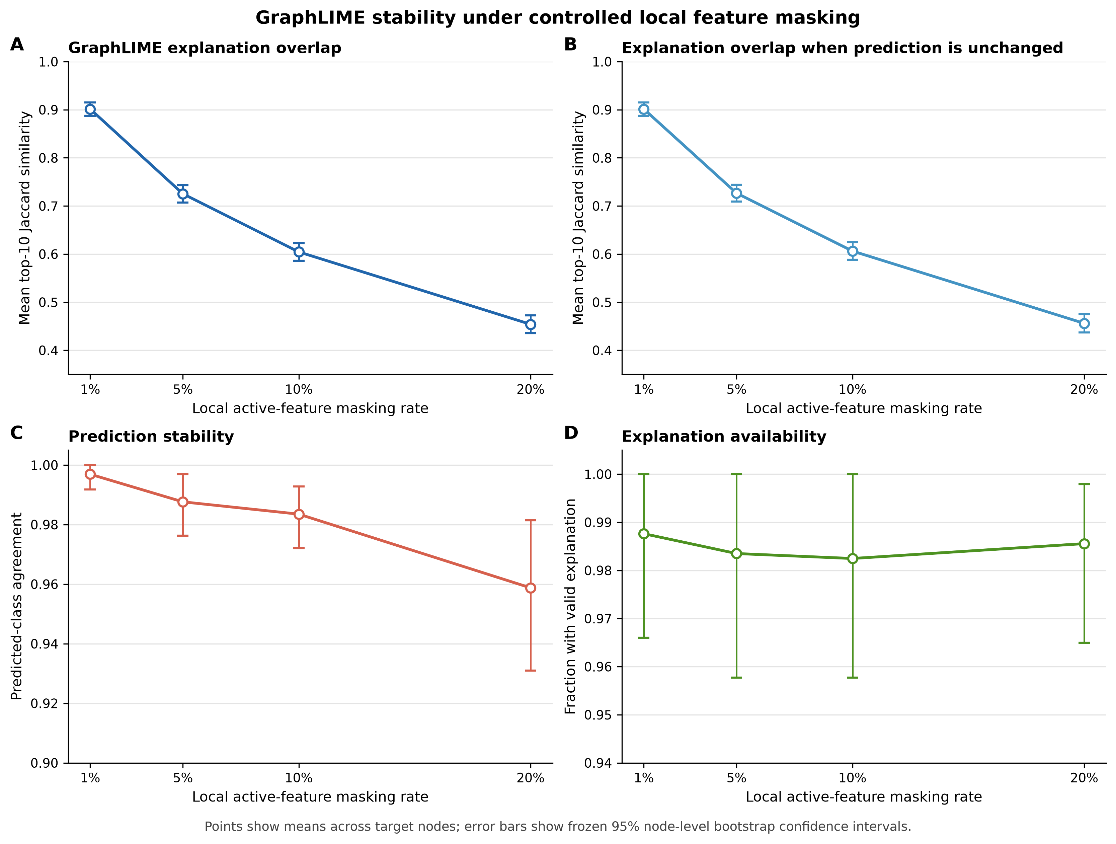
\includegraphics[width=\linewidth,height=0.8\textheight,keepaspectratio]{./media/image1.png}

\textbf{Fig. 1} Explanation and prediction stability across
feature-masking rates. Points show means across target nodes; error bars
show frozen 95\% node-level bootstrap confidence intervals.

The reduction in explanation overlap was apparent across the complete
range of masking conditions rather than being confined to the most
severe perturbation. Relative to the mean Jaccard similarity of 0.9015
at 1\% masking, the mean had decreased to 0.7253 at 5\% and 0.6045 at
10\%, before reaching 0.4541 at 20\%. At the highest masking rate, the
mean top-10 explanation therefore shared substantially less of its
selected feature set with the corresponding baseline explanation than
under the lowest masking condition. Figure 1 summarizes this
rate-dependent pattern together with the frozen 95\% node-level
bootstrap confidence intervals.

The paired endpoint analysis provided further evidence for this
reduction. Comparing the 1\% and 20\% masking conditions within target
nodes, the mean paired change in top-10 Jaccard similarity was

\[\begin{matrix}
 & \Delta J_{0.01,0.20} = - 0.4475, & & \text{(29)}
\end{matrix}\]

with a 95\% node-level bootstrap confidence interval of
\textbf{{[}-0.4660, -0.4282{]}}. The corresponding two-sided Wilcoxon
signed-rank comparison remained significant after Holm adjustment
(\(p_{Holm} = 7.30 \times 10^{- 17}\)), with a matched-pairs
rank-biserial correlation of \textbf{-1.00} under the difference
convention defined in Section 3.7. The negative direction indicates
lower explanation overlap at 20\% masking than at 1\% masking among the
non-zero paired differences included in the signed-rank calculation.

The rate-dependent pattern was also evident at the level of individual
target nodes. Across the ordered masking rates of 1\%, 5\%, 10\%, and
20\%, \textbf{93.75\%} of eligible nodes exhibited a monotonically
non-increasing sequence of mean Jaccard similarity. The aggregate
decline in explanation overlap was therefore accompanied by a highly
consistent directional pattern across the target-node cohort, although
strict monotonicity was not observed for every node.

Taken together, these results support \textbf{H1}: top-10 GraphLIME
explanation overlap decreased as the severity of controlled feature
masking increased. The effect was substantial between the endpoint
conditions and was observed consistently across most target nodes.
Whether this decline persists when analysis is restricted specifically
to perturbations that preserve the GCN\textquotesingle s predicted class
is examined in Section 4.3.
\end{quote}

\subsection{\texorpdfstring{Stability Conditional on Prediction
Agreement
}{Stability Conditional on Prediction Agreement }}\label{stability-conditional-on-prediction-agreement}

\begin{quote}
The reduction in GraphLIME explanation stability persisted when the
analysis was restricted to perturbation observations for which the GCN
retained its baseline predicted class. Among observations satisfying
both prediction agreement and explanation availability, the mean top-10
Jaccard similarity was \textbf{0.9014} at 1\% masking, \textbf{0.7266}
at 5\%, \textbf{0.6063} at 10\%, and \textbf{0.4560} at 20\%. The
prediction-conditioned trajectory therefore closely followed the decline
observed in the unconditional explanation-stability analysis of Section
4.2.

The endpoint comparison showed a substantial decrease in explanation
overlap despite preservation of the predicted class. Between the 1\% and
20\% masking conditions, the mean paired change in
prediction-conditioned Jaccard similarity was

\[\begin{matrix}
 & \Delta J_{0.01,0.20}^{same} = - 0.4454, & & \text{(30)}
\end{matrix}\]

with a 95\% node-level bootstrap confidence interval of
\textbf{{[}-0.4637, -0.4269{]}}. The corresponding two-sided Wilcoxon
signed-rank comparison remained significant after Holm adjustment
(\(p_{Holm} = 7.30 \times 10^{- 17}\)), with a matched-pairs
rank-biserial correlation of \textbf{-1.00} under the difference
convention specified in Section 3.7.

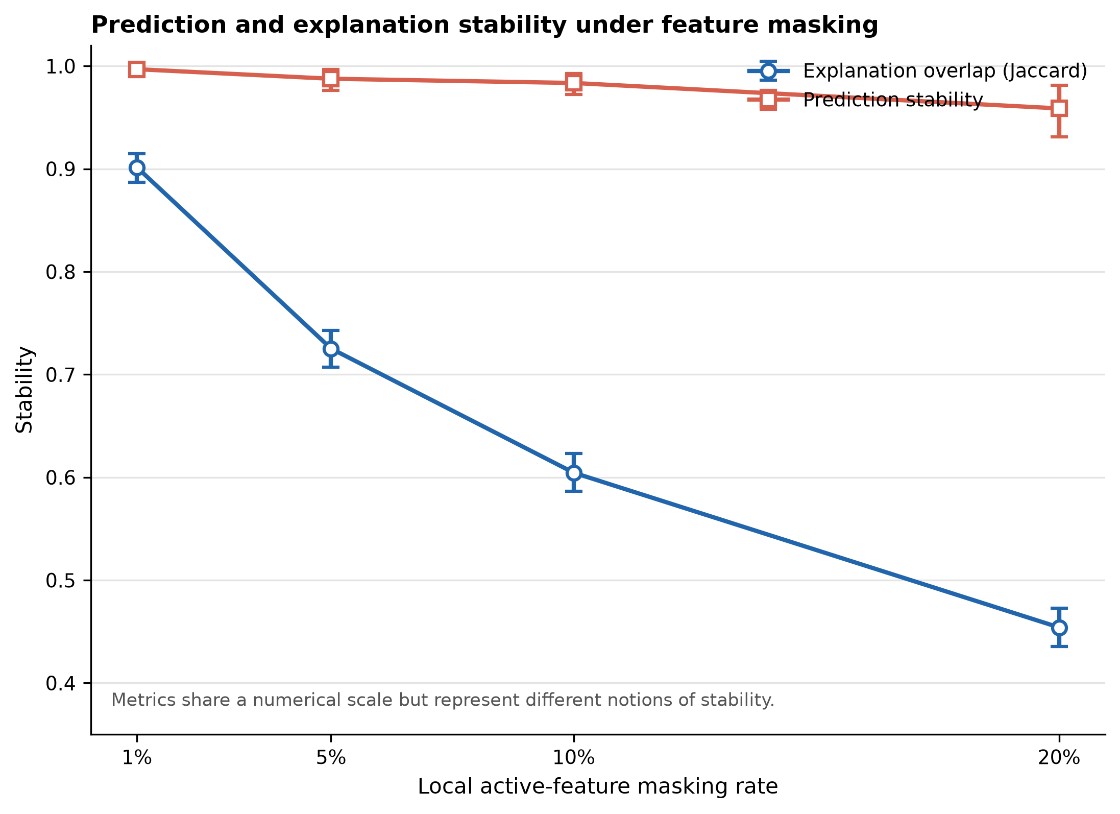
\includegraphics[width=\linewidth,height=0.8\textheight,keepaspectratio]{./media/image2.png}

\textbf{Fig. 2} Prediction and explanation stability under controlled
feature masking. Explanation overlap decreases substantially with
increasing masking severity despite comparatively high prediction
stability, illustrating that preservation of the predicted class does
not imply preservation of the corresponding GraphLIME explanation.

The directional pattern was also consistent across individual target
nodes. Across the ordered masking conditions, \textbf{92.71\%} of
eligible nodes exhibited a monotonically non-increasing sequence of mean
prediction-conditioned Jaccard similarity. As in the unconditional
analysis, this proportion indicates a highly consistent decline across
the cohort while allowing for node-specific departures from strict
monotonicity.

These results support \textbf{H2} and demonstrate that the decline in
explanation overlap cannot be accounted for solely by perturbations that
change the model\textquotesingle s predicted class. Even when analysis
was restricted to observations satisfying

\[\begin{matrix}
 & {\widehat{y}}_{r,s}(v) = {\widehat{y}}_{0}(v), & & \text{(31)}
\end{matrix}
\]

the features selected by GraphLIME became progressively less similar to
the baseline explanation as masking severity increased. Preservation of
the categorical prediction was therefore compatible with substantial
changes in the corresponding local feature explanation.

The distinction is also visible when the prediction-conditioned and
unconditional explanation-stability trajectories are compared. At 20\%
masking, for example, the unconditional mean Jaccard similarity was
\textbf{0.4541}, whereas the prediction-conditioned mean was
\textbf{0.4560}. The small numerical difference between these summaries
indicates that restricting the analysis to prediction-preserving
observations did not materially alter the observed rate-dependent
decline in explanation overlap. This comparison is descriptive; it was
not treated as a separate inferential hypothesis.

The results therefore establish the central empirical phenomenon
motivating the study: \textbf{prediction preservation does not imply
explanation preservation} under the controlled feature perturbations
considered here. The extent to which changes in prediction stability and
explanation stability are coupled across target nodes is examined
directly in Section 4.4.
\end{quote}

\subsection{Prediction--Explanation Stability
Coupling}\label{predictionexplanation-stability-coupling}

\begin{quote}
The preceding analyses showed that explanation overlap decreased
substantially with increasing feature masking, including when the GCN
retained its baseline predicted class. To examine whether changes in
predictive and explanatory stability were coupled at the target-node
level, endpoint changes between the 1\% and 20\% masking conditions were
compared for the 97 nodes with valid measurements at both endpoints.

Across these nodes, mean prediction stability decreased by
\textbf{0.0381} between the endpoint conditions, whereas mean
explanation stability decreased by \textbf{0.4475}. Thus, the magnitude
of the observed change in top-10 explanation overlap was considerably
larger than the corresponding change in the proportion of perturbation
repetitions preserving the predicted class. These quantities measure
different outcomes and are not interpreted as directly commensurate
effect sizes; rather, their contrasting endpoint behaviour motivates
examination of their node-level association.

The association between the two endpoint changes was weak. As defined in
Section 3.7, let \(\Delta P(v)\)denote the change in prediction
stability and \(\Delta J(v)\)the change in explanation stability between
1\% and 20\% masking. Across the 97 endpoint-valid nodes, the
descriptive Spearman correlation was

\[\begin{matrix}
 & \rho_{S}\left( \Delta,P\Delta J \right) = - 0.0271, & & \text{(32)}
\end{matrix}
\]

while the descriptive Pearson correlation was

\[\begin{matrix}
 & r\left( \Delta,P\Delta J \right) = 0.0927. & & \text{(33)}
\end{matrix}
\]

Both coefficients were close to zero, indicating little observed
node-level correspondence between the magnitude of change in prediction
stability and the magnitude of change in explanation overlap within this
experiment. As specified in Section 3.7, these correlations were treated
descriptively; no independent-and-identically-distributed correlation
significance test was applied because the target nodes originate from a
single graph and their neighbourhoods may overlap.

A particularly prominent form of this divergence occurred among nodes
whose endpoint prediction-stability proportion did not change.
\textbf{Eighty-six of the 97 nodes (88.66\%)} had the same
prediction-stability proportion at 1\% and 20\% masking while
simultaneously exhibiting a decrease in mean explanation overlap. In
this analysis, an unchanged endpoint prediction-stability proportion
means that the fraction of the ten perturbation repetitions preserving
the baseline predicted class was equal at the two endpoint masking
rates. It does \textbf{not} imply that every individual perturbation
realization preserved the prediction or that identical perturbation
outcomes occurred at both rates.

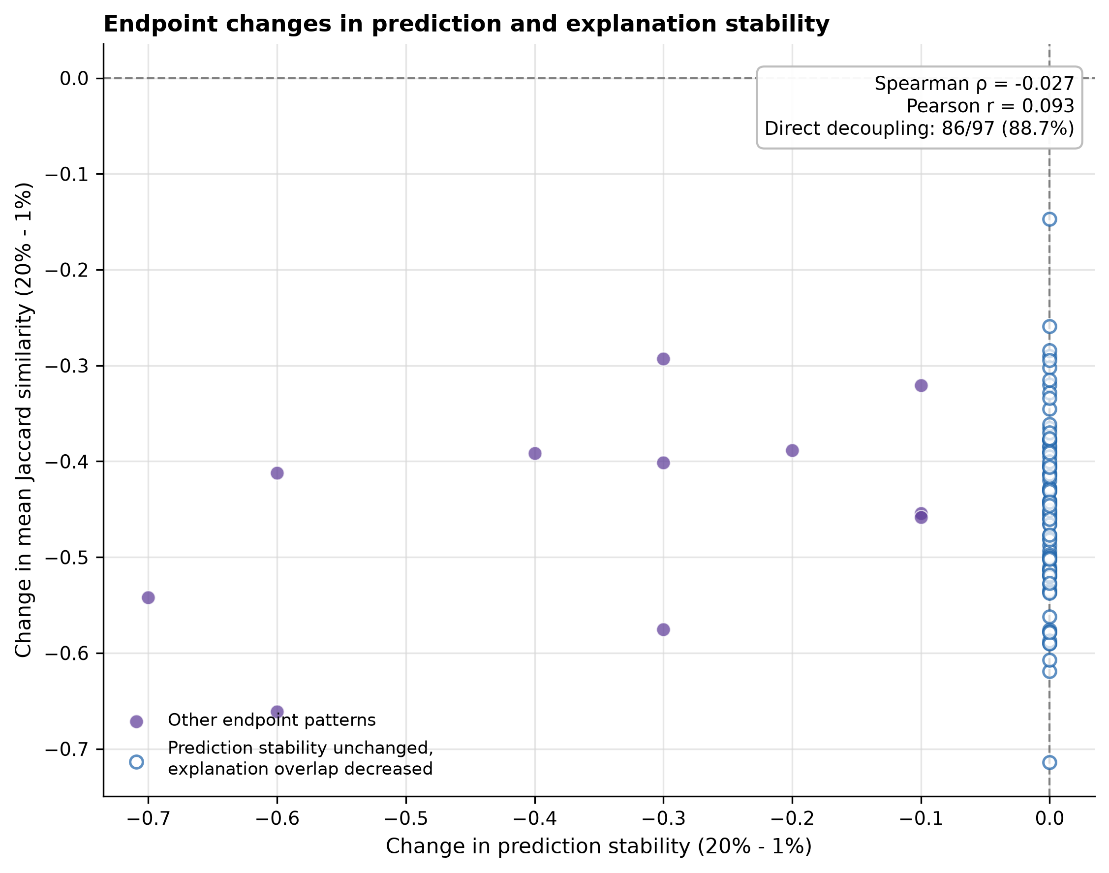
\includegraphics[width=\linewidth,height=0.8\textheight,keepaspectratio]{./media/image3.png}

\textbf{Fig. 3} Endpoint coupling between prediction and explanation
stability from 1\% to 20\% feature masking. Each point represents a
target node and shows the change in prediction-stability proportion
against the corresponding change in mean top-10 Jaccard explanation
overlap. The vertical concentration at zero indicates nodes whose
endpoint prediction-stability proportion was unchanged, while negative
explanation-stability changes indicate reduced explanation overlap.

Figure 3 visualizes the joint endpoint changes in prediction and
explanation stability. The concentration of observations around
\(\Delta P(v) = 0\), together with predominantly negative values of
\(\Delta J(v)\), illustrates the principal empirical pattern: for many
target nodes, explanation overlap declined even though the aggregate
proportion of prediction-preserving perturbations remained unchanged
between the endpoint conditions.

These findings support \textbf{H4}, which proposed that prediction and
explanation stability would not be perfectly coupled. Within the fixed
Cora experiment, changes in prediction stability provided little
indication of the corresponding magnitude of changes in GraphLIME
explanation overlap. The result complements the prediction-conditioned
analysis in Section 4.3 by showing at the target-node level that
explanatory stability can deteriorate substantially without a
corresponding deterioration in the measured proportion of stable
predictions.
\end{quote}

\subsection{\texorpdfstring{Explanation Availability
}{Explanation Availability }}\label{explanation-availability}

\begin{quote}
GraphLIME explanation availability remained high across all four
feature-masking conditions. Of the \textbf{3,880} perturbation
observations, \textbf{3,821 (98.48\%)} produced valid perturbed
explanations, while \textbf{59 (1.52\%)} were unavailable. As specified
in Section 3.6, unavailable explanations were analysed separately and
their Jaccard similarities were treated as missing rather than assigned
a value of zero.

The number of unavailable explanations was \textbf{12} at 1\% masking,
\textbf{16} at 5\%, \textbf{17} at 10\%, and \textbf{14} at 20\%.
Because each masking condition contained 970 perturbation observations,
these counts correspond to unavailability rates of approximately
\textbf{1.24\%, 1.65\%, 1.75\%, and 1.44\%}, respectively. Equivalently,
explanation availability was approximately \textbf{98.76\%, 98.35\%,
98.25\%, and 98.56\%} across the four masking rates. Figure 4 summarizes
the rate-specific pattern.

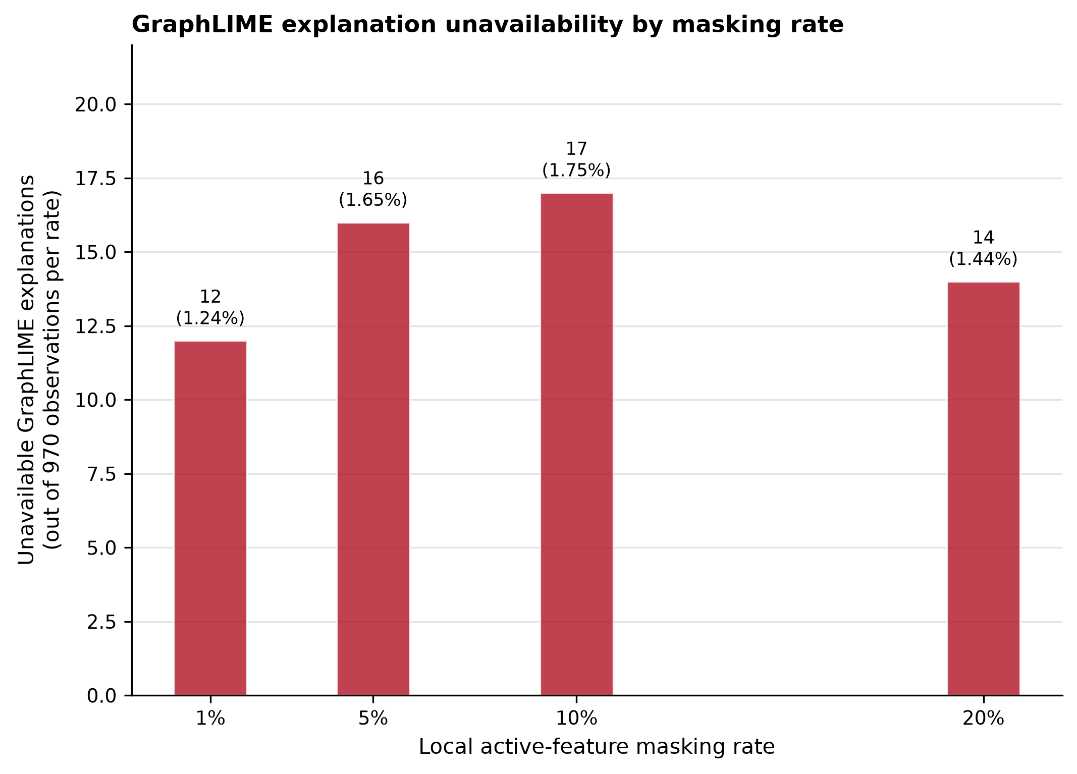
\includegraphics[width=\linewidth,height=0.8\textheight,keepaspectratio]{./media/image4.png}

\textbf{Fig. 4} GraphLIME explanation unavailability across
feature-masking rates. Bars show the proportion of perturbation
observations for which a complete top-10 perturbed explanation was
unavailable. Unavailability remained low across all masking conditions
and did not increase monotonically with masking severity.

Importantly, explanation unavailability did \textbf{not} increase
monotonically with masking severity. Although the number of unavailable
explanations increased from 12 at 1\% masking to 17 at 10\%, it
subsequently decreased to 14 at 20\%. The observed rate-wise pattern
therefore did not support the directional expectation specified in
\textbf{H5} that explanation unavailability would increase as
perturbation severity increased.

The 59 unavailable perturbed explanations were associated with two
recorded failure modes. In \textbf{35 observations}, the fitted
GraphLIME solution contained fewer than the 10 non-zero coefficients
required to construct a complete top-10 explanation. The remaining
\textbf{24 observations} were classified as optimizer non-convergence.
These cases were retained in the diagnostic record and were not
converted into artificial explanation-overlap values.

The distinction between explanation unavailability and explanation
disagreement is important for interpreting the preceding stability
results. A valid perturbed explanation with low Jaccard similarity
indicates that GraphLIME successfully produced an explanation whose
selected features differed substantially from the baseline set. An
unavailable explanation instead indicates that a complete top-10
explanation could not be obtained under the predefined validity
criteria. Treating both outcomes as \(J = 0\) would therefore conflate
explanation change with explanation failure. The high overall
availability observed here indicates that the declining Jaccard
similarities reported in Sections 4.2-4.4 were calculated predominantly
from successfully obtained perturbed explanations rather than being
driven by unavailable cases.

Overall, explanation availability remained above \textbf{98\% at every
masking rate}, while explanation overlap declined substantially as
masking severity increased. The experiment therefore provided mixed
evidence across the stability dimensions considered: feature masking
produced a pronounced rate-dependent reduction in explanation overlap,
but it did not produce a corresponding monotonic deterioration in the
ability of GraphLIME to return a complete explanation. Accordingly,
\textbf{H5 was not supported by the observed rate-wise availability
pattern}.

Table 2. Stability outcomes across feature-masking rates
\end{quote}

{\def\LTcaptype{none} % do not increment counter
\begin{longtable}[]{@{}
  >{\raggedright\arraybackslash}p{(\linewidth - 8\tabcolsep) * \real{0.1756}}
  >{\raggedright\arraybackslash}p{(\linewidth - 8\tabcolsep) * \real{0.1854}}
  >{\raggedright\arraybackslash}p{(\linewidth - 8\tabcolsep) * \real{0.1971}}
  >{\raggedright\arraybackslash}p{(\linewidth - 8\tabcolsep) * \real{0.1638}}
  >{\raggedright\arraybackslash}p{(\linewidth - 8\tabcolsep) * \real{0.1864}}@{}}
\toprule\noalign{}
\begin{minipage}[b]{\linewidth}\raggedright
\textbf{Masking rate}
\end{minipage} & \begin{minipage}[b]{\linewidth}\raggedright
\textbf{Prediction stability}
\end{minipage} & \begin{minipage}[b]{\linewidth}\raggedright
\textbf{Explanation availability}
\end{minipage} & \begin{minipage}[b]{\linewidth}\raggedright
\textbf{Mean top-10 Jaccard}
\end{minipage} & \begin{minipage}[b]{\linewidth}\raggedright
\textbf{Mean Jaccard given prediction agreement}
\end{minipage} \\
\midrule\noalign{}
\endhead
\bottomrule\noalign{}
\endlastfoot
1\% & 0.9969 & 0.9876 & 0.9015 & 0.9014 \\
5\% & 0.9876 & 0.9835 & 0.7253 & 0.7266 \\
10\% & 0.9835 & 0.9825 & 0.6045 & 0.6063 \\
20\% & 0.9588 & 0.9856 & 0.4541 & 0.4560 \\
\end{longtable}
}

\begin{quote}
\textbf{Table 2} Summary of predictive and explanatory stability across
feature-masking conditions. Prediction stability denotes the proportion
of perturbation observations preserving the baseline predicted class.
Explanation availability denotes the proportion yielding a valid
complete top-10 GraphLIME explanation. Jaccard similarity is calculated
only for observations with valid explanations; unavailable explanations
are not assigned zero similarity.
\end{quote}

\section{\texorpdfstring{Discussion }{Discussion }}\label{discussion}

\begin{quote}
This study investigated whether local GraphLIME feature explanations
remain stable when the input features of a frozen GCN are subjected to
controlled perturbations. The principal finding is that predictive
stability and explanation stability exhibited markedly different
behaviour under increasing feature masking. Across the four perturbation
levels, prediction agreement remained comparatively high, decreasing
from 0.9969 at 1\% masking to 0.9588 at 20\%, whereas mean top-10
explanation overlap decreased from 0.9015 to 0.4541. The
prediction-conditioned analysis produced a nearly identical decline in
explanation overlap, from 0.9014 to 0.4560. These results indicate that,
within the experimental conditions considered here, preservation of the
model\textquotesingle s categorical prediction did not imply
preservation of the corresponding local feature explanation.

The observed decline in explanation overlap supports H1 and shows that
GraphLIME explanations became progressively less stable as the magnitude
of feature perturbation increased. The endpoint decrease of 0.4475 in
mean top-10 Jaccard similarity was accompanied by a 95\% bootstrap
confidence interval that excluded zero, and 93.75\% of eligible target
nodes exhibited a monotonically non-increasing explanation-stability
trajectory across the ordered masking rates. This pattern suggests that
the aggregate decline was not attributable to a small number of
unusually unstable nodes. Instead, decreasing overlap was observed
across a large majority of the evaluated target-node cohort. The result
is relevant to the broader evaluation of post-hoc GNN explanations
because robustness to small changes in the explained input has been
identified as an important property of reliable explanation methods
{[}2, 3{]}. Recent surveys of GNN explainability similarly distinguish
explanation robustness and stability from conventional measures of
predictive performance {[}2{]}.

The prediction-conditioned results provide an important qualification to
this finding. Under H2, explanation overlap was evaluated only for
perturbation observations in which the GCN retained its baseline
predicted class. Nevertheless, mean Jaccard similarity declined from
0.9014 at 1\% masking to 0.4560 at 20\%, with a mean paired endpoint
change of -0.4454. This decline was almost identical in magnitude to
that obtained without conditioning on prediction agreement.
Consequently, explanation instability in this experiment cannot be
attributed solely to cases in which feature perturbation caused the
model to cross a decision boundary and change its predicted class.
Instead, substantial changes in the selected explanatory features were
observed even among perturbations for which the categorical model
decision was preserved.

This distinction is consistent with a broader concern in explanation
robustness research: predictive invariance and explanatory invariance
are different properties. Previous work has shown that explanations of
neural models can be sensitive to small input perturbations, motivating
robustness and stability as evaluation dimensions in their own right
{[}2, 3{]}. In the graph domain, Li et al. demonstrated that GNN
explanations can change substantially under limited structural
perturbations while model predictions remain correct, illustrating that
predictive behaviour alone does not guarantee explanation robustness
{[}9{]}. The present study examines a different setting --
non-adversarial feature masking rather than adversarial structural
modification -- but the observed separation between prediction
preservation and explanation preservation is compatible with this
broader distinction. The current results should therefore be interpreted
as evidence for this phenomenon specifically within the controlled
GraphLIME experiment, rather than as a direct replication of adversarial
robustness results.

The prediction-stability results under H3 further clarify this
separation. Prediction agreement decreased with masking severity, with a
mean endpoint change of -0.0381 between 1\% and 20\% masking. Thus, the
perturbations were not entirely behaviourally neutral: stronger feature
masking produced some deterioration in prediction stability. However,
the scale of the observed change differed substantially from the
simultaneous decrease in explanation overlap. At 20\% masking,
prediction stability remained 0.9588, while mean explanation overlap had
fallen to 0.4541. These values should not be interpreted as directly
comparable effect sizes because they quantify different properties. They
nevertheless demonstrate that high aggregate prediction agreement can
coexist with substantially lower agreement between the features selected
by the local explanation procedure.

The node-level coupling analysis under H4 provides additional evidence
that the two forms of stability were not tightly linked in this
experiment. Across the 97 endpoint-valid target nodes, the descriptive
Spearman correlation between endpoint changes in prediction and
explanation stability was -0.0271, while the Pearson correlation was
0.0927. Both values were close to zero. Moreover, 86 of 97 nodes
(88.66\%) had an unchanged prediction-stability proportion between the
1\% and 20\% masking conditions while exhibiting decreased explanation
overlap. The latter result is particularly informative because it
demonstrates that a node need not show a deterioration in its aggregate
rate of prediction preservation for its explanation overlap to decline.
As emphasized in Section 4.4, however, equality of endpoint
prediction-stability proportions does not imply identical prediction
outcomes for every perturbation realization.

Taken together, H1-H4 therefore point to a common empirical conclusion:
explanation stability constituted a distinct behaviour that was not
captured adequately by prediction stability alone. This observation has
implications for the evaluation of post-hoc GNN explainers. Evaluating
an explanation method only on instances for which the underlying model
is accurate or prediction-stable may leave an additional source of
variability unexamined. Contemporary evaluations of GNN explainability
increasingly recognize robustness as a separate criterion alongside
properties such as correctness, usability, and computational
characteristics {[}2{]}. The results of the present study support the
practical value of explicitly measuring explanation stability under
controlled perturbations rather than treating stable predictions as a
proxy for stable explanations.

H5 produced a different result and provides an important counterpoint to
the explanation-overlap findings. Explanation availability remained
above 98\% at every masking rate, and the rate of unavailable
explanations did not increase monotonically with perturbation severity.
The unavailable counts were 12, 16, 17, and 14 at masking rates of 1\%,
5\%, 10\%, and 20\%, respectively. H5 was therefore not supported. This
result indicates that the primary stability effect was not a simple
consequence of GraphLIME increasingly failing to return explanations
under stronger perturbation. In most perturbation observations, a
complete explanation remained available; what changed substantially was
the identity of the features appearing in that explanation.

This distinction between explanation availability and explanation
stability is methodologically important. An unavailable explanation
represents a failure to obtain a complete top-10 feature set under the
predefined criteria, whereas a valid explanation with low Jaccard
similarity represents a successfully generated explanation that differs
from its baseline counterpart. Conflating these cases by assigning zero
similarity to unavailable explanations would artificially combine two
different phenomena. By retaining unavailable cases as missing for
overlap calculations and analysing availability separately, the present
design isolates changes in explanation composition from failures of
explanation generation. The high availability rates observed across all
four masking conditions strengthen the interpretation that the decline
in Jaccard similarity reflects changes among successfully generated
explanations rather than an increasing prevalence of failed
explanations.

One possible explanation for the observed sensitivity lies in the local
nature of GraphLIME itself. GraphLIME constructs feature-wise kernels
from the local graph neighbourhood and estimates sparse feature
importance through an HSIC-Lasso objective {[}7{]}. Masking active
feature entries changes the local feature distributions from which these
kernels are constructed. Consequently, even when the frozen GCN remains
on the same side of its categorical decision boundary, the statistical
relationships represented within the local GraphLIME optimization
problem can change. The selected sparse feature set may therefore change
without requiring a change in the predicted class. This interpretation
follows from the structure of the method and is consistent with the
experimental observations, but the present experiments do not identify a
unique causal mechanism for the instability. Establishing whether
changes arise primarily from kernel construction, sparse feature
competition, local neighbourhood characteristics, or interactions among
these factors would require additional targeted experiments.

The results should also not be interpreted as showing that GraphLIME is
generally unreliable. Stability is only one property of an explanation
method, and sensitivity to perturbed inputs is not necessarily
equivalent to incorrectness. In particular, if a perturbation changes
information that the model uses internally while leaving the final
argmax class unchanged, a changed explanation may reflect a genuine
alteration in the model\textquotesingle s local behaviour rather than an
error by the explainer. Conversely, an explanation method that remains
unchanged under every perturbation would not necessarily be desirable if
the model\textquotesingle s internal dependence on features has
genuinely changed. The present experiment therefore measures empirical
explanation stability; it does not establish a ground-truth threshold at
which an explanation should be regarded as correct or incorrect.

This consideration also limits the interpretation of the top-10 Jaccard
metric. Jaccard similarity captures membership agreement between
selected feature sets, but it does not represent changes in coefficient
magnitude or feature ranking within the overlapping set. Two
explanations may therefore obtain high Jaccard similarity while
assigning substantially different importance coefficients to the same
features, or obtain lower similarity because features near the selection
boundary exchange positions. Accordingly, the current top-10 analysis
provides a deliberately interpretable measure of set-level stability
rather than a complete characterization of explanation variation.

Within these boundaries, the study provides evidence that prediction
stability alone is insufficient for characterizing the behaviour of
local GraphLIME explanations under feature perturbation. The strongest
result is not merely that explanation overlap decreased as masking
increased, but that this decrease persisted after conditioning on
prediction agreement and exhibited little node-level coupling with
changes in prediction stability. At the same time, explanation
availability remained high and showed no monotonic deterioration.
Together, these findings separate three properties that can otherwise be
conflated: whether a prediction is preserved, whether an explanation can
be generated, and whether the generated explanation remains similar to
its baseline form. For the fixed Cora graph, frozen GCN, and GraphLIME
configuration studied here, these properties behaved differently under
controlled feature masking.

The broader implication is that robustness evaluation of post-hoc GNN
explanations benefits from treating explanation behaviour as an object
of evaluation in its own right. Recent GNN-explainability literature
identifies robustness and stability as continuing challenges and
evaluation considerations {[}2, 3{]}. The present results contribute a
controlled empirical case study of this issue for GraphLIME: stable
categorical predictions and high explanation availability can coexist
with substantial changes in the selected local explanatory features.
Whether the same pattern generalizes across datasets, GNN architectures,
explanation methods, perturbation operators, and alternative stability
metrics remains an empirical question and motivates the limitations and
future research directions considered in Section 6.
\end{quote}

\section{\texorpdfstring{Limitations }{Limitations }}\label{limitations}

\begin{quote}
The findings of this study should be interpreted within the boundaries
of its controlled experimental design. The study was designed to isolate
the relationship between feature perturbation, prediction stability, and
GraphLIME explanation stability rather than to establish general
conclusions about all graph neural networks or graph explanation
methods. Several limitations therefore define the scope within which the
results should be understood.

First, the experiments were conducted on a \textbf{single
citation-network dataset, Cora}. Cora provides a well-established
setting for node-classification experiments, but its graph structure,
sparse node features, class distribution, and neighbourhood
characteristics represent only one type of attributed graph. Explanation
behaviour may differ on larger graphs, graphs with denser or continuous
node attributes, heterophilous networks, heterogeneous graphs, or graphs
from other application domains. The observed decrease in GraphLIME
explanation overlap should therefore be interpreted as an empirical
result for the fixed Cora setting rather than as evidence that the same
quantitative behaviour will occur across graph datasets.

Second, the predictive model was restricted to \textbf{one two-layer GCN
architecture and one validation-selected checkpoint}. Freezing the model
was important for the present experimental design because it ensured
that changes observed after perturbation could not be attributed to
model retraining or parameter variation. However, this control also
limits the generality of the findings. Different GNN architectures may
encode and aggregate feature information differently, potentially
producing different relationships between feature perturbation and
explanation stability. Architectures based on attention, alternative
message-passing operators, different neighbourhood depths, or other
graph-learning mechanisms may therefore exhibit different stability
characteristics. Similarly, the present study does not quantify
variability across independently trained instances of the same GCN
architecture.

Third, the explanation analysis considered \textbf{GraphLIME only}.
GraphLIME constructs local feature explanations using
neighbourhood-based kernels and a sparse HSIC-Lasso objective, and the
stability patterns observed here may depend partly on these
methodological characteristics. Other GNN explanation methods can target
different explanatory objects, including nodes, edges, subgraphs, or
continuous feature attributions, and may respond differently to the same
perturbations. Consequently, the results should not be generalized from
GraphLIME to post-hoc GNN explainers as a whole. A comparative study
applying a common perturbation protocol to multiple explanation methods
would be required to determine whether the observed separation between
prediction and explanation stability is method-specific or more broadly
shared.

Fourth, the perturbation analysis was intentionally restricted to
\textbf{feature masking}. Only active feature entries within the frozen
two-hop explanation neighbourhood were eligible for masking; graph
connectivity, model parameters, and all other experimental components
remained unchanged. This design provides a controlled test of
sensitivity to feature information but does not characterize robustness
to structural perturbations such as edge addition, edge deletion, node
removal, or neighbourhood modification. It also does not consider
alternative feature perturbations such as additive noise, continuous
feature displacement, feature replacement, or distribution-aware
corruption. Different perturbation operators can represent substantially
different changes to the input and may therefore produce different
explanation-stability behaviour.

The masking protocol itself introduces an additional scope constraint.
Perturbed active entries were set to zero without subsequent feature
re-normalization, and masks at different perturbation rates were sampled
separately rather than constructed as nested extensions of lower-rate
masks. These choices were fixed before the perturbation analysis and
applied consistently to all target nodes. They allow each masking
condition to represent a separately sampled perturbation at the
specified severity, but they also mean that differences between adjacent
rates do not correspond to progressively enlarging the same feature
mask. The results therefore characterize stability under the particular
randomized masking protocol used in this study.

Fifth, explanation stability was primarily quantified using
\textbf{top-10 Jaccard similarity}. This measure provides a transparent
assessment of membership agreement between the baseline and perturbed
feature sets, but it discards information about coefficient magnitudes
and within-set feature rankings. For example, two explanations
containing the same ten features receive a Jaccard similarity of one
even if their estimated importance coefficients differ substantially.
Conversely, replacement of a feature near the top-10 selection boundary
reduces set overlap even when the underlying coefficient values are
similar. The current results therefore characterize \textbf{set-level
feature-selection stability}, not every possible dimension of
explanation stability. Rank-based measures, coefficient-distance
measures, or stability analyses across multiple values of \(K\) could
provide complementary perspectives.

Relatedly, the choice of \(K = 10\) fixes the resolution at which
explanation overlap was evaluated. This value was held constant
throughout the study to ensure comparability across target nodes and
perturbation conditions, but stability may depend on explanation-set
size. Smaller values of \(K\) could emphasize changes among the most
highly weighted features, whereas larger values could produce different
overlap behaviour by including lower-ranked coefficients. The study did
not conduct a post-hoc sensitivity analysis over multiple values of
\(K\), because doing so after observing the primary results would alter
the scope of the frozen experimental protocol.

Sixth, the statistical analysis is constrained by the \textbf{dependence
structure of a single graph}. The target node was treated as the
statistical unit, and perturbation repetitions were aggregated within
node rather than treated as independent observations. Node-level
bootstrap confidence intervals and paired node-level comparisons were
used accordingly. Nevertheless, target nodes belong to the same Cora
graph and their local neighbourhoods may overlap, so independence
between target-node observations cannot be assumed strictly. The
node-level procedure avoids the substantially stronger and inappropriate
assumption that all 3,880 perturbation observations are independent, but
it does not eliminate dependence induced by shared graph structure.
Inferential quantities should therefore be interpreted as summaries of
the fixed experimental graph rather than as population-level guarantees
across independently sampled graphs.

Seventh, each node-masking-rate condition was evaluated using
\textbf{ten perturbation seeds}. Repeated perturbations provide
information about variability induced by random masking, but ten
realizations constitute a finite sample of the possible masks available
for each target node and masking severity. Prediction-stability
proportions are consequently discrete at the node level, and
explanation-stability estimates may vary if substantially more
perturbation realizations are evaluated. Increasing the number of
perturbation seeds would permit finer estimation of within-node
perturbation variability, although at increased computational cost
because each perturbation requires recomputation of both the frozen GNN
output and the local GraphLIME explanation.

Eighth, the GraphLIME implementation reproduces the \textbf{HSIC-Lasso
objective} used by GraphLIME but does not reproduce the original
optimization algorithm exactly. The original GraphLIME formulation
employs non-negative least-angle regression for solving the sparse
optimization problem, whereas the implementation in this study uses a
\textbf{non-negative proximal-gradient procedure} applied to the same
constrained convex objective. Numerical validation was therefore
performed explicitly: all 97 retained baseline solutions satisfied the
predefined KKT validation criteria, with residuals below the specified
tolerance where applicable. These checks support the numerical
consistency of the solutions with the implemented objective, but they do
not establish algorithmic equivalence between proximal-gradient
optimization and the original non-negative LARS procedure. Accordingly,
the present results should be described as an objective-faithful
GraphLIME implementation rather than an exact reproduction of the
original optimizer.

Ninth, explanation availability was determined using predefined
computational validity criteria, including convergence of the
optimization procedure and the availability of at least ten non-zero
coefficients for constructing a complete top-10 explanation. Of the
3,880 perturbation observations, 59 explanations were unavailable under
these criteria. Their Jaccard similarities were retained as missing
rather than assigned a value of zero. This treatment avoids conflating
explanation-generation failure with explanation disagreement, but it
also means that overlap statistics are conditional on explanation
availability. Because availability exceeded 98\% at every masking rate,
the amount of missing explanation-overlap data was limited;
nevertheless, the stability summaries do not describe the unavailable
observations themselves.

Finally, the study does not possess \textbf{ground-truth feature
explanations} against which GraphLIME outputs can be evaluated. A change
in the selected explanatory feature set cannot therefore be classified
automatically as either desirable adaptation or erroneous instability.
Feature masking may genuinely alter aspects of the frozen
GCN\textquotesingle s local behaviour without changing its final
predicted class, in which case a changed explanation could reflect a
meaningful change in the model rather than a failure of the explanation
method. Conversely, explanation changes could also arise from
sensitivity of the local surrogate construction or sparse
feature-selection procedure. The present experiments distinguish and
quantify explanation stability, prediction stability, and explanation
availability, but they do not establish explanation correctness or
causal faithfulness.

These limitations define the appropriate interpretation of the study
rather than invalidate its controlled findings. Within a fixed Cora
graph, frozen two-layer GCN, fixed GraphLIME configuration,
predetermined target-node cohort, and preregistered feature-masking
protocol, the experiments provide consistent evidence that top-10
explanation overlap decreases with increasing masking severity and that
this decrease persists when the predicted class is preserved. At the
same time, explanation availability remains high and does not
deteriorate monotonically. Establishing the extent to which these
observations generalize will require experiments across additional
graphs, model architectures, explanation methods, perturbation
operators, explanation metrics, and independently trained models.
\end{quote}

\section{Conclusions}\label{conclusions}

\begin{quote}
This study investigated the stability of local GraphLIME feature
explanations for a frozen graph neural network under controlled
perturbations of the input node features. The central objective was to
determine whether preservation of a GNN prediction is accompanied by
preservation of its corresponding local explanation. Using the Cora
citation network, a frozen two-layer GCN, a fixed GraphLIME
configuration, and predetermined feature-masking conditions, the study
evaluated prediction stability, top-10 explanation stability, and
explanation availability as distinct empirical properties.

The results showed a pronounced reduction in explanation stability as
feature-masking severity increased. Mean top-10 Jaccard similarity
between baseline and perturbed GraphLIME explanations decreased from
\textbf{0.9015 at 1\% masking to 0.4541 at 20\% masking}, while
prediction stability decreased more modestly from \textbf{0.9969 to
0.9588}. Importantly, the decline in explanation overlap persisted when
the analysis was restricted to perturbation observations that preserved
the baseline predicted class: prediction-conditioned mean Jaccard
similarity decreased from \textbf{0.9014 to 0.4560} across the same
masking range. These findings demonstrate that, within the experimental
setting considered here, preservation of the categorical prediction did
not imply preservation of the selected explanatory feature set.

The node-level analysis further supported this distinction. Changes in
prediction stability and explanation stability between the endpoint
masking conditions exhibited little descriptive association, with
Spearman and Pearson correlations close to zero. Moreover, \textbf{86 of
97 endpoint-valid target nodes (88.66\%)} retained the same endpoint
prediction-stability proportion while exhibiting decreased explanation
overlap. Prediction stability therefore provided limited information
about the corresponding change in GraphLIME explanation stability within
this experiment.

Explanation availability exhibited a different pattern. Complete
GraphLIME explanations remained available for more than \textbf{98\% of
perturbation observations at every masking rate}, and unavailability did
not increase monotonically with perturbation severity. Consequently, the
observed reduction in explanation overlap was not accompanied by a
corresponding systematic deterioration in the ability of the explanation
procedure to return a complete top-10 feature set. This distinction
reinforces the importance of treating \textbf{prediction preservation,
explanation preservation, and explanation availability as separate
properties} when evaluating post-hoc explanations.

The contribution of this study is therefore a controlled empirical
characterization of GraphLIME explanation stability rather than a claim
that GraphLIME explanations are generally unreliable. Explanation change
does not by itself establish explanation incorrectness, particularly
because no ground-truth feature explanations were available and a
perturbation may alter aspects of local model behaviour without changing
the final predicted class. The conclusions are also bounded to the fixed
Cora graph, GCN checkpoint, GraphLIME configuration, feature-masking
protocol, and top-10 set-based stability measure used in this study.

Future work can determine whether the observed separation between
predictive and explanatory stability extends beyond this experimental
setting. Relevant directions include evaluating additional graph
datasets and GNN architectures, comparing multiple explanation methods,
examining structural and alternative feature perturbations, varying
explanation-set size, incorporating rank- and coefficient-sensitive
stability measures, increasing the number of perturbation repetitions,
and studying independently trained model instances. Such extensions
would help establish when explanation instability reflects genuine
changes in model behaviour and when it instead arises from sensitivity
of the explanation procedure itself.

Overall, the findings demonstrate that \textbf{stable predictions alone
are insufficient to characterize the stability of local GraphLIME
explanations}. Under controlled feature masking, the frozen GCN
frequently preserved its categorical prediction while the corresponding
explanatory feature sets changed substantially. Explicit evaluation of
explanation stability therefore provides information about post-hoc GNN
explanations that cannot be obtained from predictive stability alone.
\end{quote}

\section{\texorpdfstring{Data and Code Availability
}{Data and Code Availability }}\label{data-and-code-availability}

\begin{quote}
The dataset used in this study is the publicly available \textbf{Cora
citation-network dataset}, accessed through the Planetoid dataset
interface in PyTorch Geometric. The experimental code, configuration
files, frozen model checkpoint, processed experimental results,
statistical-analysis outputs, and figures required to reproduce and
inspect the reported analyses are publicly available in the accompanying
GitHub repository:

\href{https://github.com/ngclara07/graphlime-stability}{GraphLIME
Explanation Stability Study -- GitHub repository}

The repository documents the complete experimental pipeline, including
baseline GCN training and checkpoint selection, target-node selection,
GraphLIME explanation generation and numerical validation, controlled
feature perturbation, perturbation-result validation, statistical
analysis, hypothesis evaluation, and figure generation. Raw
perturbation-level results and the derived node-level and rate-level
summaries used in the manuscript are retained in the repository to
support reproducibility and independent inspection of the reported
findings.

The experimental protocol and principal analysis artifacts were frozen
after validation. Subsequent manuscript preparation did not involve
retraining the GCN, replacing target nodes, retuning GraphLIME
hyperparameters, modifying the perturbation protocol, or altering the
statistical analysis in response to the observed results.
\end{quote}

\section{References}\label{references}

\begin{quote}
{[}1{]} Kipf, T.N., Welling, M.: Semi-supervised classification with
graph convolutional networks. In: International Conference on Learning
Representations (ICLR) (2017).

{[}2{]} Li, X., Wang, J., Yan, Z.: Can graph neural networks be
adequately explained? A survey. ACM Computing Surveys 57(5), Article
131, 1-36 (2025). \url{https://doi.org/10.1145/3711122}

{[}3{]} Ma, W., Liu, X., Liu, Y., Ma, Y.: Post-hoc explainability of
graph neural networks: A comprehensive survey. Information Sciences 740,
123202 (2026). \url{https://doi.org/10.1016/j.ins.2026.123202}

{[}4{]} Ying, Z., Bourgeois, D., You, J., Zitnik, M., Leskovec, J.:
GNNExplainer: Generating explanations for graph neural networks. In:
Advances in Neural Information Processing Systems, vol. 32 (2019).

{[}5{]} Luo, D., Cheng, W., Xu, D., Yu, W., Zong, B., Chen, H., Zhang,
X.: Parameterized explainer for graph neural network. In: Advances in
Neural Information Processing Systems, vol. 33 (2020).

{[}6{]} Yuan, H., Yu, H., Wang, J., Li, K., Ji, S.: On explainability of
graph neural networks via subgraph explorations. In: Proceedings of the
38th International Conference on Machine Learning, Proceedings of
Machine Learning Research, vol. 139, pp. 12241-12252 (2021).

{[}7{]} Huang, Q., Yamada, M., Tian, Y., Singh, D., Chang, Y.:
GraphLIME: Local interpretable model explanations for graph neural
networks. IEEE Transactions on Knowledge and Data Engineering 35(7),
6968-6972 (2023). \url{https://doi.org/10.1109/TKDE.2022.3187455}

{[}8{]} Agarwal, C., Queen, O., Lakkaraju, H., Zitnik, M.: Evaluating
explainability for graph neural networks. Scientific Data 10, 144
(2023). \url{https://doi.org/10.1038/s41597-023-01974-x}

{[}9{]} Li, J., Pang, M., Dong, Y., Jia, J., Wang, B.: Graph neural
network explanations are fragile. In: Proceedings of the 41st
International Conference on Machine Learning, Proceedings of Machine
Learning Research, vol. 235, pp. 28551-28567 (2024).

{[}10{]} Amara, K., Ying, R., Zhang, Z.: GraphFramEx: Towards systematic
evaluation of explainability methods for graph neural networks. In:
Proceedings of the First Learning on Graphs Conference, Proceedings of
Machine Learning Research, vol. 198 (2022).

{[}11{]} Yamada, M., Jitkrittum, W., Sigal, L., Xing, E.P., Sugiyama,
M.: High-dimensional feature selection by feature-wise kernelized Lasso.
Neural Computation 26(1), 185-207 (2014).
\url{https://doi.org/10.1162/NECO_a_00537}

{[}12{]} Sen, P., Namata, G., Bilgic, M., Getoor, L., Gallagher, B.,
Eliassi-Rad, T.: Collective classification in network data. AI Magazine
29(3), 93-106 (2008). \url{https://doi.org/10.1609/aimag.v29i3.2157}

{[}13{]} Fey, M., Lenssen, J.E.: Fast graph representation learning with
PyTorch Geometric. In: ICLR Workshop on Representation Learning on
Graphs and Manifolds (2019).

{[}14{]} Kingma, D.P., Ba, J.: Adam: A method for stochastic
optimization. In: International Conference on Learning Representations
(ICLR) (2015).

{[}15{]} Jaccard, P.: Étude comparative de la distribution florale dans
une portion des Alpes et du Jura. Bulletin de la Société Vaudoise des
Sciences Naturelles 37, 547-579 (1901).
\url{https://doi.org/10.5169/seals-266450}

{[}16{]} Efron, B., Tibshirani, R.J.: An Introduction to the Bootstrap.
Chapman \& Hall, New York (1993).

{[}17{]} Wilcoxon, F.: Individual comparisons by ranking methods.
Biometrics Bulletin 1(6), 80-83 (1945).
\url{https://doi.org/10.2307/3001968}

{[}18{]} Holm, S.: A simple sequentially rejective multiple test
procedure. Scandinavian Journal of Statistics 6(2), 65-70 (1979).

{[}19{]} Kerby, D.S.: The simple difference formula: An approach to
teaching nonparametric correlation. Comprehensive Psychology 3, Article
1 (2014). \url{https://doi.org/10.2466/11.IT.3.1}
\end{quote}

\section{Appendix A Supplementary Experimental
Details}\label{appendix-a-supplementary-experimental-details}

\begin{quote}
This appendix records supplementary implementation and reproducibility
details for the experimental procedure described in Section 3. All
settings reported here correspond to the frozen configuration used to
generate the results in Section 4. They were not modified during
subsequent statistical interpretation or manuscript preparation.

\textbf{A.1 Baseline GCN Configuration}

The predictive model was a two-layer graph convolutional network trained
on the predefined Cora training split. Model selection was performed
exclusively using validation accuracy, and the test split was evaluated
only after the selected checkpoint had been restored.

The frozen baseline configuration was:
\end{quote}

{\def\LTcaptype{none} % do not increment counter
\begin{longtable}[]{@{}
  >{\raggedright\arraybackslash}p{(\linewidth - 2\tabcolsep) * \real{0.5137}}
  >{\raggedright\arraybackslash}p{(\linewidth - 2\tabcolsep) * \real{0.4863}}@{}}
\toprule\noalign{}
\begin{minipage}[b]{\linewidth}\raggedright
\textbf{Parameter}
\end{minipage} & \begin{minipage}[b]{\linewidth}\raggedright
\textbf{Value}
\end{minipage} \\
\midrule\noalign{}
\endhead
\bottomrule\noalign{}
\endlastfoot
Dataset & Cora \\
Dataset interface & PyTorch Geometric Planetoid \\
Feature preprocessing & NormalizeFeatures \\
Model & Two-layer GCN \\
Hidden dimension & 16 \\
Activation & ReLU \\
Dropout probability & 0.5 \\
Optimizer & Adam \\
Learning rate & 0.01 \\
Weight decay & 0.0005 \\
Maximum training epochs & 200 \\
Training/model seed & 42 \\
Selected checkpoint epoch & 125 \\
Training accuracy at selected checkpoint & 0.9929 \\
Validation accuracy at selected checkpoint & 0.7840 \\
Test accuracy after checkpoint selection & 0.8060 \\
\end{longtable}
}

\begin{quote}
The selected model parameters were subsequently frozen. No retraining or
fine-tuning was performed during explanation generation or feature
perturbation.

\textbf{A.2 Target-Node Selection and Baseline Explanation Cohort}

After restoration of the frozen GCN checkpoint, correctly classified
nodes from the predefined test split were identified. A deterministic
random permutation with selection seed 42 was used to select 100
correctly classified test nodes without replacement. The selected node
set was fixed before GraphLIME explanation validity was assessed and was
not modified in response to subsequent experimental outcomes.

Of the 100 predetermined target nodes, 97 admitted valid baseline
GraphLIME explanations. Three nodes---2697, 2625, and 2411---were
classified as output-degenerate because the local GCN probability
vectors did not provide sufficient variation for construction of a
non-degenerate GraphLIME output kernel. These nodes were retained in the
diagnostic record and were not replaced. The resulting 97
baseline-explainable nodes formed the fixed cohort for the perturbation
study.

All 97 retained baseline explanation problems converged with at least 10
non-zero feature coefficients. Numerical validation of the implemented
constrained HSIC-Lasso solutions produced 97 of 97 KKT validation
passes. The maximum active-set stationarity residual was
\textbf{\(6.59 \times 10^{-7}\)}, the maximum inactive-set violation was
\textbf{0}, the minimum inactive-set slack was
\textbf{\(2.80 \times 10^{-5}\)}, and the maximum complementarity
residual was \textbf{\(3.79 \times 10^{-7}\)}.

\textbf{A.3 Frozen GraphLIME Configuration}

GraphLIME explanations were constructed from the two-hop neighbourhood
of each target node. The complete GCN class-probability vectors were
used to construct the local output kernel. Gaussian kernels were
constructed for locally varying input features and for model outputs,
with bandwidth determined from the median positive pairwise Euclidean
distance of the corresponding local variable.

The frozen explanation configuration was:
\end{quote}

{\def\LTcaptype{none} % do not increment counter
\begin{longtable}[]{@{}
  >{\raggedright\arraybackslash}p{(\linewidth - 2\tabcolsep) * \real{0.4830}}
  >{\raggedright\arraybackslash}p{(\linewidth - 2\tabcolsep) * \real{0.4794}}@{}}
\toprule\noalign{}
\begin{minipage}[b]{\linewidth}\raggedright
\textbf{Parameter}
\end{minipage} & \begin{minipage}[b]{\linewidth}\raggedright
\textbf{Value}
\end{minipage} \\
\midrule\noalign{}
\endhead
\bottomrule\noalign{}
\endlastfoot
Neighbourhood depth & 2 hops \\
Explanation size & Top 10 features \\
Regularization parameter (\(\rho\)) & 0.03 \\
Candidate (\(\rho\)) values used during calibration & 0.001, 0.003, 0.01, 0.03,
0.1, 0.3 \\
Calibration cohort & First 10 frozen selected target nodes \\
Optimizer & Non-negative proximal-gradient \\
Maximum optimizer iterations & 10,000 \\
Relative coefficient-change tolerance & \(1x10^{- 8}\) \\
Coefficient zero tolerance & \(1x10^{- 8}\) \\
KKT validation tolerance & \(1x10^{- 8}\) \\
Kernel & Gaussian \\
Kernel centring & Yes \\
Frobenius normalization & Yes \\
\end{longtable}
}

\begin{quote}
The regularization parameter was selected before the perturbation
experiments. A candidate was eligible only when optimization converged
and at least 10 non-zero coefficients were available for every
calibration node. The selected value, \textbf{\(\rho = 0.03\)}, was then held
fixed for all remaining baseline and perturbed explanations.

The implementation solves the non-negative HSIC-Lasso objective used by
GraphLIME through proximal-gradient optimization. It is therefore
objective-faithful to the stated convex formulation but does not
constitute an exact optimizer-level reproduction of the original
non-negative least-angle regression procedure.

\textbf{A.4 Feature-Masking Protocol}

Perturbations were restricted to active feature entries within the same
two-hop neighbourhood used for the target node\textquotesingle s
GraphLIME explanation. An entry was eligible for masking only when its
value in the original normalized feature matrix was non-zero.

For a target node with \textbf{n\_active} eligible local entries and
masking rate \textbf{r}, the number of masked entries was

\[m(r) = min\text{\{}n_{active},max\left( 1,\left\lfloor r\ n_{active} + 0.5 \right\rfloor \right)\text{\}}\ \]

The frozen perturbation configuration was:
\end{quote}

{\def\LTcaptype{none} % do not increment counter
\begin{longtable}[]{@{}
  >{\raggedright\arraybackslash}p{(\linewidth - 2\tabcolsep) * \real{0.4834}}
  >{\raggedright\arraybackslash}p{(\linewidth - 2\tabcolsep) * \real{0.4790}}@{}}
\toprule\noalign{}
\begin{minipage}[b]{\linewidth}\raggedright
\textbf{Parameter}
\end{minipage} & \begin{minipage}[b]{\linewidth}\raggedright
\textbf{Value}
\end{minipage} \\
\midrule\noalign{}
\endhead
\bottomrule\noalign{}
\endlastfoot
Perturbation type & Active feature masking \\
Masking rates & 1\%, 5\%, 10\%, 20\% \\
Perturbation seeds & 101-110 \\
Repetitions per node-rate condition & 10 \\
Baseline-explainable target nodes & 97 \\
Total perturbation observations & 3,880 \\
Graph structure modified & No \\
GCN retrained after perturbation & No \\
Post-mask feature renormalization & No \\
Perturbations accumulated across rates & No \\
Masks nested across rates & No \\
\end{longtable}
}

\begin{quote}
Every perturbation observation was generated from a fresh copy of the
original normalized feature matrix. Entries selected by the mask were
set to zero. Masks at different rates were sampled separately rather
than constructed by progressively extending a lower-rate mask.

Random mask generation was deterministic for each combination of target
node, masking rate, and perturbation seed. The implementation derived
the random seed as

\[s_{derived} = \left( s \times 1,000,003 + v \times 10,007 + i_{r} \times 101 \right)\backslash bmod\left( 2^{63} - 1 \right)\]

where \textbf{s} is the perturbation seed, \textbf{v} is the target-node
identifier, and \textbf{\(i_r\)} is the masking-rate index.

\textbf{A.5 Statistical Configuration}

The target node was treated as the primary statistical unit. The ten
perturbation realizations associated with each node-rate condition were
treated as repeated measurements within that node rather than as
independent observations.
\end{quote}

{\def\LTcaptype{none} % do not increment counter
\begin{longtable}[]{@{}
  >{\raggedright\arraybackslash}p{(\linewidth - 2\tabcolsep) * \real{0.4816}}
  >{\raggedright\arraybackslash}p{(\linewidth - 2\tabcolsep) * \real{0.4808}}@{}}
\toprule\noalign{}
\begin{minipage}[b]{\linewidth}\raggedright
\textbf{Analysis setting}
\end{minipage} & \begin{minipage}[b]{\linewidth}\raggedright
\textbf{Frozen value}
\end{minipage} \\
\midrule\noalign{}
\endhead
\bottomrule\noalign{}
\endlastfoot
Primary statistical unit & Target node \\
Bootstrap resamples & 10,000 \\
Bootstrap confidence level & 95\% \\
Bootstrap seed & 20260917 \\
Bootstrap interval & Percentile \\
Paired inferential test & Two-sided Wilcoxon signed-rank \\
Wilcoxon implementation & Tie-corrected normal approximation \\
Continuity correction & No \\
Zero paired differences & Excluded from signed-rank calculation \\
Multiple-comparison adjustment & Holm procedure \\
Effect-size summary & Matched-pairs rank-biserial correlation \\
H4 association measures & Pearson and Spearman correlations \\
H4 correlation significance test & None; correlations treated
descriptively \\
\end{longtable}
}

\begin{quote}
Unavailable perturbed explanations were retained as missing for
explanation-overlap calculations and were analysed separately through
explanation-availability statistics. They were never assigned a Jaccard
similarity of zero.

\textbf{A.6 Explanation Availability and Diagnostic Outcomes}

Across the 3,880 perturbation observations, 3,821 produced valid
complete top-10 perturbed explanations and 59 were unavailable. The
rate-specific diagnostic outcomes were:
\end{quote}

{\def\LTcaptype{none} % do not increment counter
\begin{longtable}[]{@{}
  >{\raggedright\arraybackslash}p{(\linewidth - 6\tabcolsep) * \real{0.2076}}
  >{\raggedright\arraybackslash}p{(\linewidth - 6\tabcolsep) * \real{0.2467}}
  >{\raggedright\arraybackslash}p{(\linewidth - 6\tabcolsep) * \real{0.2466}}
  >{\raggedright\arraybackslash}p{(\linewidth - 6\tabcolsep) * \real{0.2637}}@{}}
\toprule\noalign{}
\begin{minipage}[b]{\linewidth}\raggedright
\textbf{Masking rate}
\end{minipage} & \begin{minipage}[b]{\linewidth}\raggedright
\textbf{Total observations}
\end{minipage} & \begin{minipage}[b]{\linewidth}\raggedright
\textbf{Unavailable explanations}
\end{minipage} & \begin{minipage}[b]{\linewidth}\raggedright
\textbf{Unavailability rate}
\end{minipage} \\
\midrule\noalign{}
\endhead
\bottomrule\noalign{}
\endlastfoot
1\% & 970 & 12 & 1.24\% \\
5\% & 970 & 16 & 1.65\% \\
10\% & 970 & 17 & 1.75\% \\
20\% & 970 & 14 & 1.44\% \\
Total & 3,880 & 59 & 1.52\% \\
\end{longtable}
}

\begin{quote}
Of the 59 unavailable explanations, 35 contained fewer than the 10
non-zero coefficients required to construct a complete top-10 feature
set, while 24 were classified as optimizer non-convergence. These
outcomes were retained as diagnostic information rather than converted
into explanation-disagreement scores.

\textbf{A.7 Reproducibility and Research Artifacts}

The experimental repository preserves the frozen model checkpoint,
configuration records, baseline explanation outputs, perturbation-level
observations, validation outputs, statistical summaries, and manuscript
figures. The principal analysis artifacts include node-rate summaries,
prediction-conditioned summaries, paired rate contrasts, hypothesis
summaries, explanation-availability summaries, and endpoint coupling
analyses.

The complete research artifact is publicly available in the accompanying
repository:

\href{https://github.com/ngclara07/graphlime-stability}{GraphLIME
Explanation Stability Study -- GitHub repository}

The experimental pipeline was frozen after validation and statistical
analysis. Manuscript preparation did not involve replacing target nodes,
retraining the predictive model, retuning GraphLIME using perturbation
outcomes, modifying the masking protocol, or changing the statistical
procedures in response to the final results.
\end{quote}

\end{document}
